% INT4096 Group Project -- final report
% Build: latexmk -pdf main.tex   (see README.md in this directory)
%
% Every reported number is either (a) pulled from a generated macro in
% generated/numbers.tex, or (b) inside a table generated from run artifacts by
% scripts/build_latex_assets.py. Nothing empirical is typed by hand.
\documentclass[11pt,a4paper]{article}

\usepackage[T1]{fontenc}
\usepackage[utf8]{inputenc}
\usepackage{lmodern}
\usepackage[margin=2.5cm]{geometry}
\usepackage{microtype}
\usepackage{amsmath,amssymb}
\usepackage{booktabs}
\usepackage{siunitx}
\usepackage{graphicx}
\usepackage{xcolor}
\usepackage{caption}
\usepackage{enumitem}
\usepackage{titlesec}
\usepackage{fancyhdr}
\usepackage[hidelinks]{hyperref}
\usepackage{natbib}
\usepackage{tikz}
\usetikzlibrary{arrows.meta,positioning,shapes.geometric,fit,backgrounds}

\sisetup{detect-all}

\captionsetup{font=small,labelfont=bf,width=0.94\linewidth}
\setlist{itemsep=2pt,topsep=3pt,parsep=0pt}

% Section headings: compact, no decorative rules.
\titleformat{\section}{\normalfont\large\bfseries}{\thesection}{0.6em}{}
\titleformat{\subsection}{\normalfont\normalsize\bfseries}{\thesubsection}{0.5em}{}
\titlespacing*{\section}{0pt}{1.05em}{0.45em}
\titlespacing*{\subsection}{0pt}{0.75em}{0.3em}

\pagestyle{fancy}
\fancyhf{}
\fancyhead[L]{\footnotesize INT4096: Learning ML Through Financial Forecasting}
\fancyhead[R]{\footnotesize\thepage}
\renewcommand{\headrulewidth}{0.3pt}

% ---------------------------------------------------------------------------
% Author block: the five group members, in the order recorded in
% docs/project/responsibilities.md. Student IDs are deliberately NOT printed
% here or committed to the repository; Moodle collects them separately.
% Override without editing the source if the order must change:
%   pdflatex "\def\GroupAuthors{...}% INT4096 Group Project -- final report
% Build: latexmk -pdf main.tex   (see README.md in this directory)
%
% Every reported number is either (a) pulled from a generated macro in
% generated/numbers.tex, or (b) inside a table generated from run artifacts by
% scripts/build_latex_assets.py. Nothing empirical is typed by hand.
\documentclass[11pt,a4paper]{article}

\usepackage[T1]{fontenc}
\usepackage[utf8]{inputenc}
\usepackage{lmodern}
\usepackage[margin=2.5cm]{geometry}
\usepackage{microtype}
\usepackage{amsmath,amssymb}
\usepackage{booktabs}
\usepackage{siunitx}
\usepackage{graphicx}
\usepackage{xcolor}
\usepackage{caption}
\usepackage{enumitem}
\usepackage{titlesec}
\usepackage{fancyhdr}
\usepackage[hidelinks]{hyperref}
\usepackage{natbib}
\usepackage{tikz}
\usetikzlibrary{arrows.meta,positioning,shapes.geometric,fit,backgrounds}

\sisetup{detect-all}

\captionsetup{font=small,labelfont=bf,width=0.94\linewidth}
\setlist{itemsep=2pt,topsep=3pt,parsep=0pt}

% Section headings: compact, no decorative rules.
\titleformat{\section}{\normalfont\large\bfseries}{\thesection}{0.6em}{}
\titleformat{\subsection}{\normalfont\normalsize\bfseries}{\thesubsection}{0.5em}{}
\titlespacing*{\section}{0pt}{1.05em}{0.45em}
\titlespacing*{\subsection}{0pt}{0.75em}{0.3em}

\pagestyle{fancy}
\fancyhf{}
\fancyhead[L]{\footnotesize INT4096: Learning ML Through Financial Forecasting}
\fancyhead[R]{\footnotesize\thepage}
\renewcommand{\headrulewidth}{0.3pt}

% ---------------------------------------------------------------------------
% Author block: the five group members, in the order recorded in
% docs/project/responsibilities.md. Student IDs are deliberately NOT printed
% here or committed to the repository; Moodle collects them separately.
% Override without editing the source if the order must change:
%   pdflatex "\def\GroupAuthors{...}% INT4096 Group Project -- final report
% Build: latexmk -pdf main.tex   (see README.md in this directory)
%
% Every reported number is either (a) pulled from a generated macro in
% generated/numbers.tex, or (b) inside a table generated from run artifacts by
% scripts/build_latex_assets.py. Nothing empirical is typed by hand.
\documentclass[11pt,a4paper]{article}

\usepackage[T1]{fontenc}
\usepackage[utf8]{inputenc}
\usepackage{lmodern}
\usepackage[margin=2.5cm]{geometry}
\usepackage{microtype}
\usepackage{amsmath,amssymb}
\usepackage{booktabs}
\usepackage{siunitx}
\usepackage{graphicx}
\usepackage{xcolor}
\usepackage{caption}
\usepackage{enumitem}
\usepackage{titlesec}
\usepackage{fancyhdr}
\usepackage[hidelinks]{hyperref}
\usepackage{natbib}
\usepackage{tikz}
\usetikzlibrary{arrows.meta,positioning,shapes.geometric,fit,backgrounds}

\sisetup{detect-all}

\captionsetup{font=small,labelfont=bf,width=0.94\linewidth}
\setlist{itemsep=2pt,topsep=3pt,parsep=0pt}

% Section headings: compact, no decorative rules.
\titleformat{\section}{\normalfont\large\bfseries}{\thesection}{0.6em}{}
\titleformat{\subsection}{\normalfont\normalsize\bfseries}{\thesubsection}{0.5em}{}
\titlespacing*{\section}{0pt}{1.05em}{0.45em}
\titlespacing*{\subsection}{0pt}{0.75em}{0.3em}

\pagestyle{fancy}
\fancyhf{}
\fancyhead[L]{\footnotesize INT4096: Learning ML Through Financial Forecasting}
\fancyhead[R]{\footnotesize\thepage}
\renewcommand{\headrulewidth}{0.3pt}

% ---------------------------------------------------------------------------
% Author block: the five group members, in the order recorded in
% docs/project/responsibilities.md. Student IDs are deliberately NOT printed
% here or committed to the repository; Moodle collects them separately.
% Override without editing the source if the order must change:
%   pdflatex "\def\GroupAuthors{...}% INT4096 Group Project -- final report
% Build: latexmk -pdf main.tex   (see README.md in this directory)
%
% Every reported number is either (a) pulled from a generated macro in
% generated/numbers.tex, or (b) inside a table generated from run artifacts by
% scripts/build_latex_assets.py. Nothing empirical is typed by hand.
\documentclass[11pt,a4paper]{article}

\usepackage[T1]{fontenc}
\usepackage[utf8]{inputenc}
\usepackage{lmodern}
\usepackage[margin=2.5cm]{geometry}
\usepackage{microtype}
\usepackage{amsmath,amssymb}
\usepackage{booktabs}
\usepackage{siunitx}
\usepackage{graphicx}
\usepackage{xcolor}
\usepackage{caption}
\usepackage{enumitem}
\usepackage{titlesec}
\usepackage{fancyhdr}
\usepackage[hidelinks]{hyperref}
\usepackage{natbib}
\usepackage{tikz}
\usetikzlibrary{arrows.meta,positioning,shapes.geometric,fit,backgrounds}

\sisetup{detect-all}

\captionsetup{font=small,labelfont=bf,width=0.94\linewidth}
\setlist{itemsep=2pt,topsep=3pt,parsep=0pt}

% Section headings: compact, no decorative rules.
\titleformat{\section}{\normalfont\large\bfseries}{\thesection}{0.6em}{}
\titleformat{\subsection}{\normalfont\normalsize\bfseries}{\thesubsection}{0.5em}{}
\titlespacing*{\section}{0pt}{1.05em}{0.45em}
\titlespacing*{\subsection}{0pt}{0.75em}{0.3em}

\pagestyle{fancy}
\fancyhf{}
\fancyhead[L]{\footnotesize INT4096: Learning ML Through Financial Forecasting}
\fancyhead[R]{\footnotesize\thepage}
\renewcommand{\headrulewidth}{0.3pt}

% ---------------------------------------------------------------------------
% Author block: the five group members, in the order recorded in
% docs/project/responsibilities.md. Student IDs are deliberately NOT printed
% here or committed to the repository; Moodle collects them separately.
% Override without editing the source if the order must change:
%   pdflatex "\def\GroupAuthors{...}\input{main.tex}"
% ---------------------------------------------------------------------------
\providecommand{\GroupAuthors}{%
  Zhang Yancheng \quad Dong Yuankun \quad Zhang Haoyu \\
  Lau Pak Hei \quad Lui Shing Lam}

\input{generated/numbers.tex}

\title{\vspace{-1.2cm}\bfseries Learning Machine Learning Through Financial
Time-Series Forecasting:\\[2pt]
\large A Reproducible Comparison of Models and Preprocessing Strategies on
Apple and Bitcoin}
\author{\GroupAuthors\\[2pt]
\small INT4096 Artificial Intelligence and Machine Learning in Education\\
\small The Education University of Hong Kong, Semester 1, 2026--27}
\date{28 November 2026}

\begin{document}
\maketitle
\vspace{-0.6cm}

\begin{abstract}
\noindent
Financial forecasting makes generalisation, leakage and baseline comparison
checkable. We compare five models and two preprocessing variants for next-session
close prediction on Apple (AAPL) and Bitcoin (BTC) under a documented,
leakage-audited protocol. Across \NRunTotal{} runs, no model beat naive persistence
by more than \BestAAPLSkill\% (AAPL) or \BestBTCAllSkill\% (BTC), \NBelowAll{} runs
were worse, and every bootstrap interval includes zero. Experimental neural
networks showed no clear advantage. We turn this negative result into a
five-objective lesson on reading skill scores, finding leakage and understanding
scaling. Without a learner study, we make no claim of learning gains.
\end{abstract}

\vspace{0.2cm}
\input{sections/01_introduction}
\input{sections/02_background}
\input{sections/03_questions}
\input{sections/04_data}
\input{sections/05_features}
\input{sections/06_method}
\input{sections/07_models}
\input{sections/08_ablation}
\input{sections/09_results}
\input{sections/09b_experimental_dl}
\input{sections/10_education}
\input{sections/11_limitations}
\input{sections/12_learnings}
\input{sections/13_conclusion}



\section*{Acknowledgements}
\addcontentsline{toc}{section}{Acknowledgements}
\noindent The repository holds hashed data snapshots, the protocol, run manifests,
tests and the notebook. AI coding assistants (Pi with
\texttt{pi-subagents}, and Claude Code) drafted code, tests and text under a
documented protocol. Zhang Yancheng directed that work: he
set the research direction, made the final decisions, and reviewed and verified
every AI-assisted change. This work is
educational, not investment advice.

\bibliographystyle{plainnat}
\bibliography{references}

\end{document}
"
% ---------------------------------------------------------------------------
\providecommand{\GroupAuthors}{%
  Zhang Yancheng \quad Dong Yuankun \quad Zhang Haoyu \\
  Lau Pak Hei \quad Lui Shing Lam}

% GENERATED by scripts/build_latex_assets.py -- do not edit by hand.
% Measured values referenced from prose, so no number is retyped by hand.
\newcommand{\NRunTotal}{20}
\newcommand{\NValAAPL}{244}
\newcommand{\BestAAPLModel}{SVR (RBF)}
\newcommand{\BestBTCModel}{Ridge}
\newcommand{\BestAAPLSkill}{+0.52}
\newcommand{\BestBTCSkill}{+0.12}
\newcommand{\SkillAAPLLinearBaseline}{-0.50}
\newcommand{\MaeAAPLLinearBaseline}{2.92}
\newcommand{\SkillAAPLRidge}{+0.29}
\newcommand{\MaeAAPLRidge}{2.90}
\newcommand{\SkillAAPLSvr}{+0.52}
\newcommand{\MaeAAPLSvr}{2.89}
\newcommand{\SkillAAPLRandomForest}{-0.78}
\newcommand{\MaeAAPLRandomForest}{2.93}
\newcommand{\SkillAAPLHistGradientBoosting}{+0.25}
\newcommand{\MaeAAPLHistGradientBoosting}{2.90}
\newcommand{\SkillBTCLinearBaseline}{+0.05}
\newcommand{\MaeBTCLinearBaseline}{1603.59}
\newcommand{\SkillBTCRidge}{+0.12}
\newcommand{\MaeBTCRidge}{1602.39}
\newcommand{\SkillBTCSvr}{+0.08}
\newcommand{\MaeBTCSvr}{1603.13}
\newcommand{\SkillBTCRandomForest}{+0.06}
\newcommand{\MaeBTCRandomForest}{1603.37}
\newcommand{\SkillBTCHistGradientBoosting}{-0.04}
\newcommand{\MaeBTCHistGradientBoosting}{1605.02}
\newcommand{\NBelowAll}{5}
\newcommand{\NBelowPtwo}{3}
\newcommand{\BestBTCAllModel}{Linear baseline}
\newcommand{\BestBTCAllVariant}{P0}
\newcommand{\BestBTCAllSkill}{+0.26}
\newcommand{\NValBTC}{358}
\newcommand{\TrialsUsed}{10}
\newcommand{\SecondsUsed}{90}
\newcommand{\TrialsMax}{24}
\newcommand{\SecondsMax}{300}
\newcommand{\NCiTotal}{20}
\newcommand{\NCiIncludeZero}{20}
\newcommand{\SupPresent}{yes}
\newcommand{\SupNCi}{4}
\newcommand{\SupNCiZero}{4}
\newcommand{\SupLossLo}{0.676}
\newcommand{\SupLossHi}{0.697}
\newcommand{\SupSeeds}{5}
\newcommand{\SupMaxEpochs}{300}
\newcommand{\SupPatience}{20}


\title{\vspace{-1.2cm}\bfseries Learning Machine Learning Through Financial
Time-Series Forecasting:\\[2pt]
\large A Reproducible Comparison of Models and Preprocessing Strategies on
Apple and Bitcoin}
\author{\GroupAuthors\\[2pt]
\small INT4096 Artificial Intelligence and Machine Learning in Education\\
\small The Education University of Hong Kong, Semester 1, 2026--27}
\date{28 November 2026}

\begin{document}
\maketitle
\vspace{-0.6cm}

\begin{abstract}
\noindent
Financial forecasting makes generalisation, leakage and baseline comparison
checkable. We compare five models and two preprocessing variants for next-session
close prediction on Apple (AAPL) and Bitcoin (BTC) under a documented,
leakage-audited protocol. Across \NRunTotal{} runs, no model beat naive persistence
by more than \BestAAPLSkill\% (AAPL) or \BestBTCAllSkill\% (BTC), \NBelowAll{} runs
were worse, and every bootstrap interval includes zero. Experimental neural
networks showed no clear advantage. We turn this negative result into a
five-objective lesson on reading skill scores, finding leakage and understanding
scaling. Without a learner study, we make no claim of learning gains.
\end{abstract}

\vspace{0.2cm}
\section{Introduction and Educational Motivation}
\label{sec:intro}

Introductory machine learning often uses problems where better models visibly win.
Such examples can hide two questions that decide whether a model is useful:
\textbf{\emph{what did it learn}, and \emph{against what baseline}?}

Short-horizon prices are close to a random walk \citep{fama1970efficient}. A
sophisticated model can therefore lose to the rule \textbf{\emph{tomorrow's price
equals today's}}, and a learner who can explain why has understood more than a
leaderboard shows.

We compare two markets, Apple (AAPL) and Bitcoin (BTC). Our \textbf{audience} is
advanced secondary-school students, pre-university learners interested in AI, and
university students without a machine-learning major. The intended outcomes are
conceptual (Section~\ref{sec:education}).

\section{Theoretical Background}
\label{sec:background}

\paragraph{Regression and generalisation.}
We predict the close of session $t+1$ from features known at the close of session
$t$. Training error usually falls as capacity grows, so performance must be judged
on unseen data \citep{hastie2009elements}.

\paragraph{Model families.}
Ridge regression is a regularised linear model. Support vector regression with an
RBF kernel \citep{drucker1997support} predicts from weighted kernel similarities,
so it depends on distances in feature space. A random forest
\citep{breiman2001random} averages bootstrapped trees to reduce variance.
Histogram gradient boosting \citep{friedman2001gradient} fits trees sequentially
to residuals and can also fit noise.

\paragraph{Preprocessing is part of the model.}
A tree splits on $x_j < \tau$. Rescaling $x_j$ by a positive constant preserves
order, so an equivalent threshold exists. A kernel method sums squared differences
\emph{across} features, so rescaling changes which feature dominates. We test this
asymmetry in Section~\ref{sec:ablation}.

\paragraph{Ordered data and leakage.}
Random cross-validation lets a model interpolate across time and is invalid here
\citep{bergmeir2018note,roberts2017crossvalidation}. We use chronological splits
with a boundary purge. Leakage, meaning information unavailable at prediction
time, can make an evaluation optimistic \citep{kaufman2012leakage}, so we test for
it.

\section{Research Questions}
\label{sec:questions}

\begin{description}[leftmargin=1.4em,style=nextline]
  \item[RQ1.] Under identical, leakage-safe conditions, how do distinct model
  families perform against naive persistence on AAPL and BTC?
  \item[RQ2.] How do complexity, tuning and changing market conditions affect
  generalisation and error patterns?
  \item[RQ3.] To what extent do preprocessing and feature choices change forecast
  error, and does the effect depend on model family and market?
  \item[RQ4.] What do selected examples and counterexamples teach learners about
  model behaviour, evaluation and responsible interpretation?
\end{description}

Five hypotheses were fixed before any result was inspected: persistence is
competitive at this horizon (H1); AAPL is more predictable than BTC (H2); scaling
moves error more for scaling-sensitive families than for trees (H3); complexity
widens the train--validation gap (H4); features matter more than the scaler (H5).
RQ4 is answered by an artefact, not a learner study, and H1 turning out true is an
acceptable outcome.

\section{Dataset and Data Provenance}
\label{sec:data}

\textbf{Two public datasets, saved once and never edited.} Each experiment
\textbf{re-checks the SHA-256 fingerprint} and stops on a mismatch
(\repodir{data/raw}{raw data}, \repodir{data/cards}{dataset cards}).

\begin{table}[H]
\centering
\caption{Where the data came from and how many rows we use. Modelling rows exclude
the first \Warmup{} bars (feature windows not yet full) and the last bar (no next
close).}
\label{tab:dataset}
\small
\begin{tabular}{@{}L{0.20\linewidth} L{0.36\linewidth} L{0.36\linewidth}@{}}
\toprule
 & \textbf{Apple (AAPL)} & \textbf{Bitcoin (BTC/USDT)} \\
\midrule
\textbf{Source} & StockAnalysis public history API & Binance public REST API, spot \\
Endpoint & \scriptsize\url{https://stockanalysis.com/api/symbol/s/aapl/history} & \scriptsize\url{https://api.binance.com/api/v3/klines} \\
Fields & date, open, high, low, close, volume, adjusted close & open time, open, high, low, close, volume \\
\textbf{Window} & \WindowAAPL & \WindowBTC \\
Daily bars & \ObsAAPL & \ObsBTC \\
Quality checks$^{*}$ & \textbf{\QualityAAPL} & \textbf{\QualityBTC} \\
\textbf{Modelling rows} & \textbf{\RowsAAPL} & \textbf{\RowsBTC} \\
Train / validation / test & \TrainRowsAAPL{} / \ValidationRowsAAPL{} / \TestRowsAAPL & \TrainRowsBTC{} / \ValidationRowsBTC{} / \TestRowsBTC \\
\bottomrule
\end{tabular}
\par\smallskip\footnotesize
$^{*}$Duplicate dates, missing values, non-positive prices, inconsistent high, low or close, negative volume.
\end{table}

\begin{table}[H]
\centering
\caption{The two datasets differ. How we handled each difference.}
\label{tab:differences}
\small
\begin{tabular}{@{}L{0.16\linewidth} L{0.21\linewidth} L{0.19\linewidth} L{0.35\linewidth}@{}}
\toprule
Difference & AAPL & BTC & \textbf{What we did} \\
\midrule
Unit & listed share, USD & one exchange, USDT & Compare assets only by \textbf{unit-free skill} \\
Calendar & exchange sessions; \GapsAAPL{} weekend or holiday gaps & every day & Keep \textbf{each calendar}; never align rows \\
Close range & \CloseRangeAAPL & \CloseRangeBTC & Use \textbf{returns and ratios} as inputs \\
Daily volatility & \RetSdAAPL\% & \RetSdBTC\% & \textbf{Fit and score separately} \\
Adjusted price & differs on \AdjDiffPctAAPL\% of days & none & Predict the \textbf{raw close} \\
\bottomrule
\end{tabular}
\end{table}

Providers revise adjusted prices later, so they contain \textbf{information
unavailable at decision time}. No split discontinuity falls in the window (the
adjusted/raw ratio never jumps by more than 2\%), and we ignore dividends.

% Keep the generated split table here, in numbering order.
\begingroup
\let\floatingtable\table
\renewcommand{\table}[1][]{\floatingtable[H]}
\input{generated/splits_table}
\endgroup

\begin{figure}[t]
  \centering
  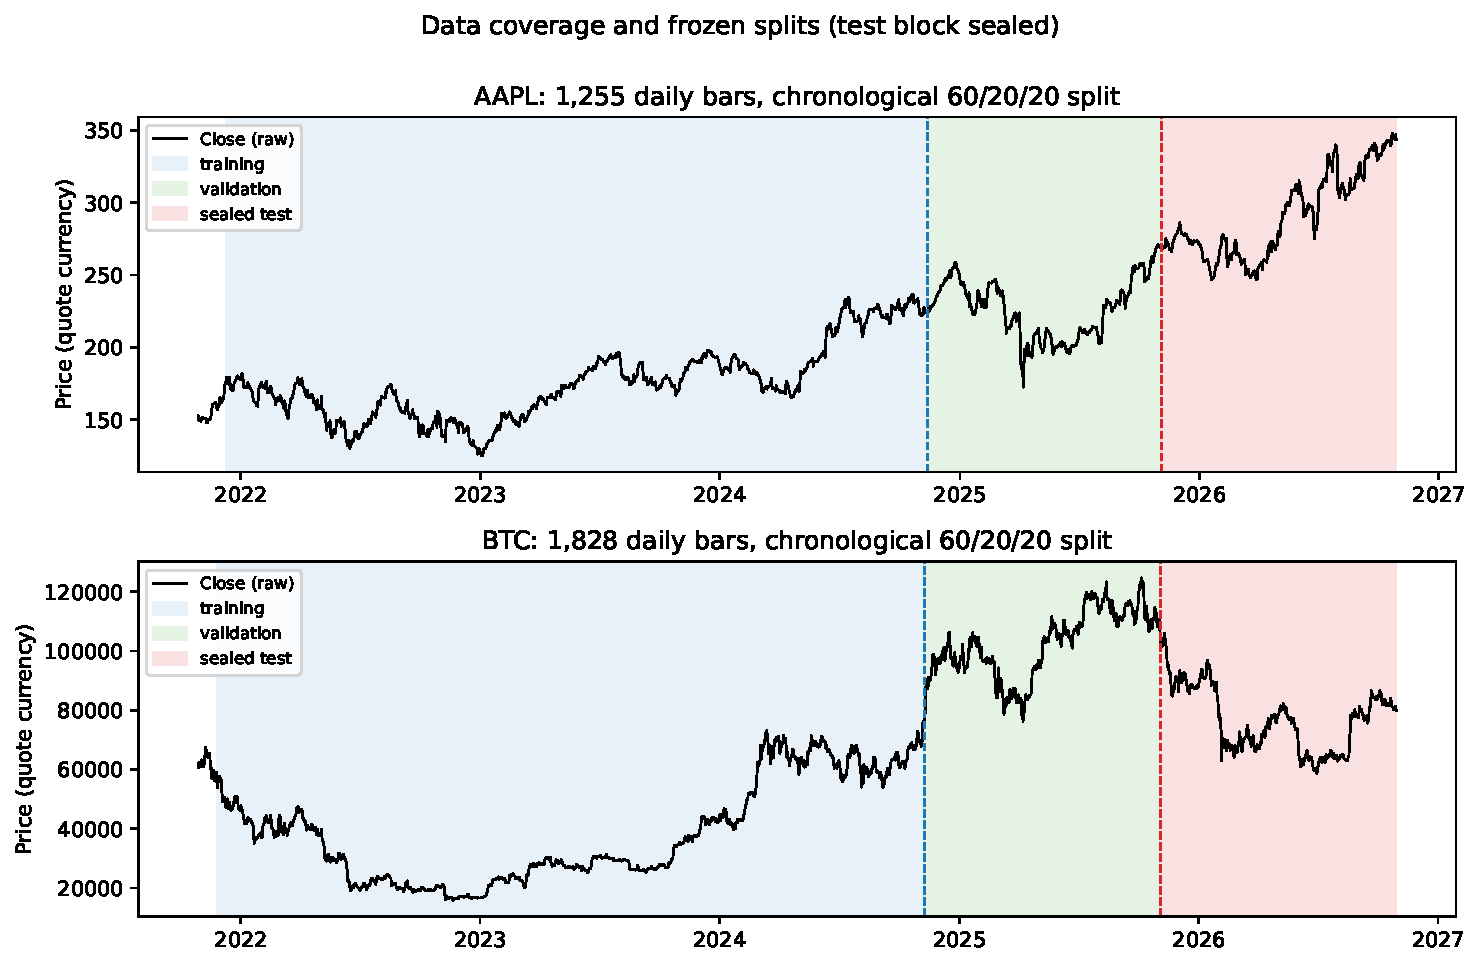
\includegraphics[width=0.9\linewidth]{figures/fig01_coverage_and_splits.pdf}
  \caption{Price history with the fixed 60/20/20 chronological split. Blue is
  training, green validation, red the \textbf{sealed test block}, which no run has
  read. The unshaded start is the feature warm-up.}
  \label{fig:coverage}
\end{figure}

\begin{figure}[t]
  \centering
  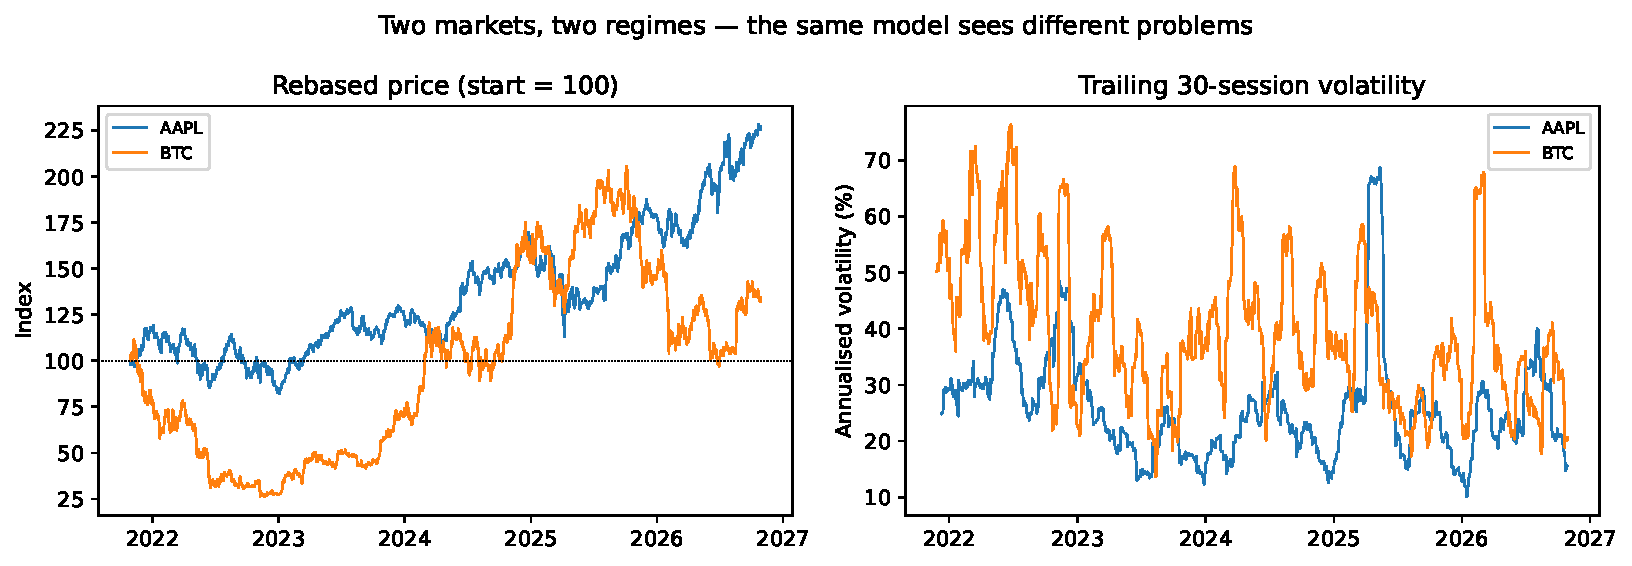
\includegraphics[width=0.9\linewidth]{figures/fig02_asset_characteristics.pdf}
  \caption{How the markets differ. Left: each series rebased to 100. Right:
  annualised 30-session volatility. BTC is usually more volatile.}
  \label{fig:assets}
\end{figure}

\section{Features and Leakage Control}
\label{sec:features}

The ten features are trailing ratios: returns over 1, 5 and 20 sessions; gaps to
5- and 20-session moving averages; realised volatility over 10 and 30 sessions;
intra-bar range; a volume anomaly; and day of week. Each uses bars up to and
including $t$, and rolling statistics require a full window.

Features are \emph{scale free} rather than price levels, which are non-stationary
and would let a model look accurate by copying today's price. The
reported quantity is error on the next close \emph{price}, while models are fitted
on the price \emph{change} and reconstructed as
$\hat{C}_{t+1} = C_t + \widehat{\Delta}_t$. The two are information-equivalent
because $C_t$ is known at decision time.

\paragraph{Boundary purge.}
With $y_t = C_{t+1}$, the last training label is a validation price and the last
validation label a sealed test price, so one row is dropped at each boundary. An
independent audit showed that, without it, perturbing one test price moved the
headline metric by 0.408 (Table~\ref{tab:splits}).

\input{generated/splits_table}

\paragraph{Enforcement.}
One test recomputes every feature from raw data with trailing formulas written
separately in the test, so a forward peek mismatches; another appends absurd future
prices and asserts earlier values are unchanged. Six canonical defects --- a
one-bar forward shift, an obfuscated equivalent, a centred window, a backward
fill, a whole-series statistic, and preprocessing fitted on train-plus-test ---
are then injected one at a time, and each must be detected.

\section{Experimental Methodology}
\label{sec:method}

Each asset is split chronologically into 60\% training, 20\% validation and 20\%
sealed test on its own session index, with a one-row purge at each boundary
(Table~\ref{tab:splits}); all models see identical boundaries and dates. Hyperparameters are chosen by random search inside an
expanding-window time-series cross-validation confined to the training block:
five folds, a one-fold gap, minimum initial training fraction 0.30. Because
tuning never sees validation, validation remains a selection holdout rather than
a second tuning set. Every family gets the same budget, \TrialsUsed{} trials and at most \SecondsUsed{}~s
per cell (the protocol caps \TrialsMax{} and \SecondsMax{}~s), and every attempted
configuration is logged.

\begin{figure}[t]
  \centering
  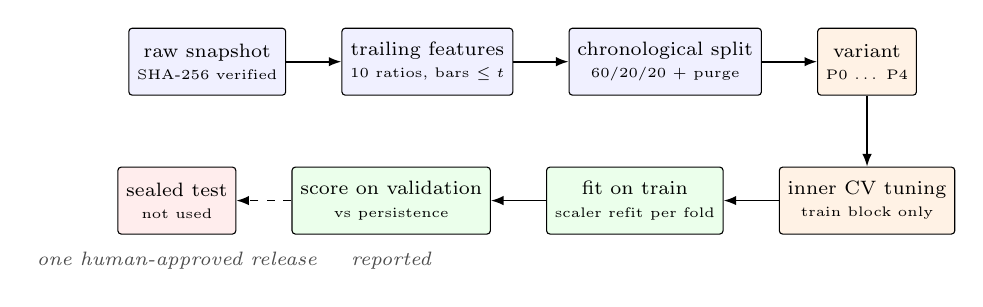
\begin{tikzpicture}[
      node distance=5mm and 7mm,
      box/.style={draw, rounded corners=1.2pt, align=center, font=\scriptsize,
                  inner sep=3pt, minimum height=8.5mm},
      arr/.style={-{Latex[length=1.6mm]}, semithick},
      lbl/.style={font=\scriptsize\itshape, text=black!70}]
    \node[box, fill=blue!6] (raw) {raw snapshot\\{\tiny SHA-256 verified}};
    \node[box, fill=blue!6, right=of raw] (feat) {trailing features\\{\tiny 10 ratios, bars $\le t$}};
    \node[box, fill=blue!6, right=of feat] (split) {chronological split\\{\tiny 60/20/20 + purge}};
    \node[box, fill=orange!10, right=of split] (pre) {variant\\{\tiny P0 \dots\ P4}};
    \node[box, fill=orange!10, below=9mm of pre] (tune) {inner CV tuning\\{\tiny train block only}};
    \node[box, fill=green!8, left=of tune] (fit) {fit on train\\{\tiny scaler refit per fold}};
    \node[box, fill=green!8, left=of fit] (eval) {score on validation\\{\tiny vs persistence}};
    \node[box, fill=red!7, left=of eval] (test) {sealed test\\{\tiny not used}};

    \draw[arr] (raw) -- (feat);
    \draw[arr] (feat) -- (split);
    \draw[arr] (split) -- (pre);
    \draw[arr] (pre) -- (tune);
    \draw[arr] (tune) -- (fit);
    \draw[arr] (fit) -- (eval);
    \draw[arr, dashed] (eval) -- (test);
    \node[lbl, below=1mm of eval] {reported};
    \node[lbl, below=1mm of test] {one human-approved release};
  \end{tikzpicture}
  \caption{The experiment pipeline, drawn to match the implementation. The scaler
  is fitted \emph{inside} the model pipeline, so it is refitted per fold and
  cannot see validation rows. Dashed arrow: the test block is not evaluated by
  any run in this report.}
  \label{fig:pipeline}
\end{figure}

We report MAE, RMSE and $R^2$, plus \emph{skill} relative to persistence on
identical forecast dates:
\begin{equation*}
  \text{skill}_{\text{MAE}} \;=\; 1 - \frac{\text{MAE}_{\text{model}}}{\text{MAE}_{\text{naive}}}.
\end{equation*}
Skill is primary because it has a meaningful zero. $R^2$ is inflated on a trending level: our naive forecast itself attains $R^2 \approx 0.96$, so a high $R^2$
here indicates a trending series, not a good model. Absolute errors are never
compared across assets. Uncertainty uses a moving-block bootstrap over consecutive dates; overlapping blocks retain dependence, so we treat it as indicative only.

\section{Model Selection and Baselines}
\label{sec:models}

The five families differ in mechanism rather than to reach a count: a
near-unregularised linear model as a learned floor, Ridge as a regularised linear
reference, RBF support vector regression as a kernel method, a random forest as a
bagged ensemble, and histogram gradient boosting as a boosted ensemble. A shallow neural network was considered and left gated: the written handout
discourages deep learning, and the instructor's reported oral guidance is recorded
as reported guidance, not as a changed rule, so that lane does not appear here.

The mandatory baseline is naive persistence, $\hat{C}_{t+1} = C_t$. It is not a straw man: for a near-random-walk series it is strong, free, and
defines the zero of the skill scale \citep{makridakis2018m4,hyndman2021fpp3}. Forecasting competitions reach the same conclusion
about simple benchmarks \citep{makridakis2018m4,hyndman2021fpp3}.

Every family is built through one shared code path, so each receives identical
feature columns in identical order and any scaler sits inside its pipeline where
it is refitted per fold. Tests assert that column identity and that a fixed seed
is deterministic.

\section{Preprocessing Ablation}
\label{sec:ablation}

RQ3 asks how much preprocessing matters. We vary one factor at a time, holding
model, features, split and tuning budget fixed; the contrast is scaling, with P0
unscaled and P2 standardised on training rows only.

\input{generated/ablation_table}

The measured pattern matches Section~\ref{sec:background}, exactly rather than
approximately: for both tree ensembles the change in validation MAE is
\emph{bit-identical} --- $0.000\%$ to printed precision --- on both assets. That is a strong internal control: had scaling moved the forests, the correct
inference would be a bug, not a discovery.

Scaling-sensitive families move slightly and not uniformly helpfully:
standardisation barely changes AAPL Ridge, worsens the AAPL linear baseline
(Table~\ref{tab:ablation}) and rescues nothing --- every value stays within about
one percentage point of the baseline. An ablation ending in no
substantial effect is a legitimate finding, and a useful teaching one: it
separates \emph{this transform changes the model} from \emph{this transform
improves the forecast}.

One variant is reported as not run: with no missing values in either snapshot an
imputation variant would duplicate the baseline cell, and we did not inject
synthetic gaps to manufacture a contrast.

\begin{figure}[t]
  \centering
  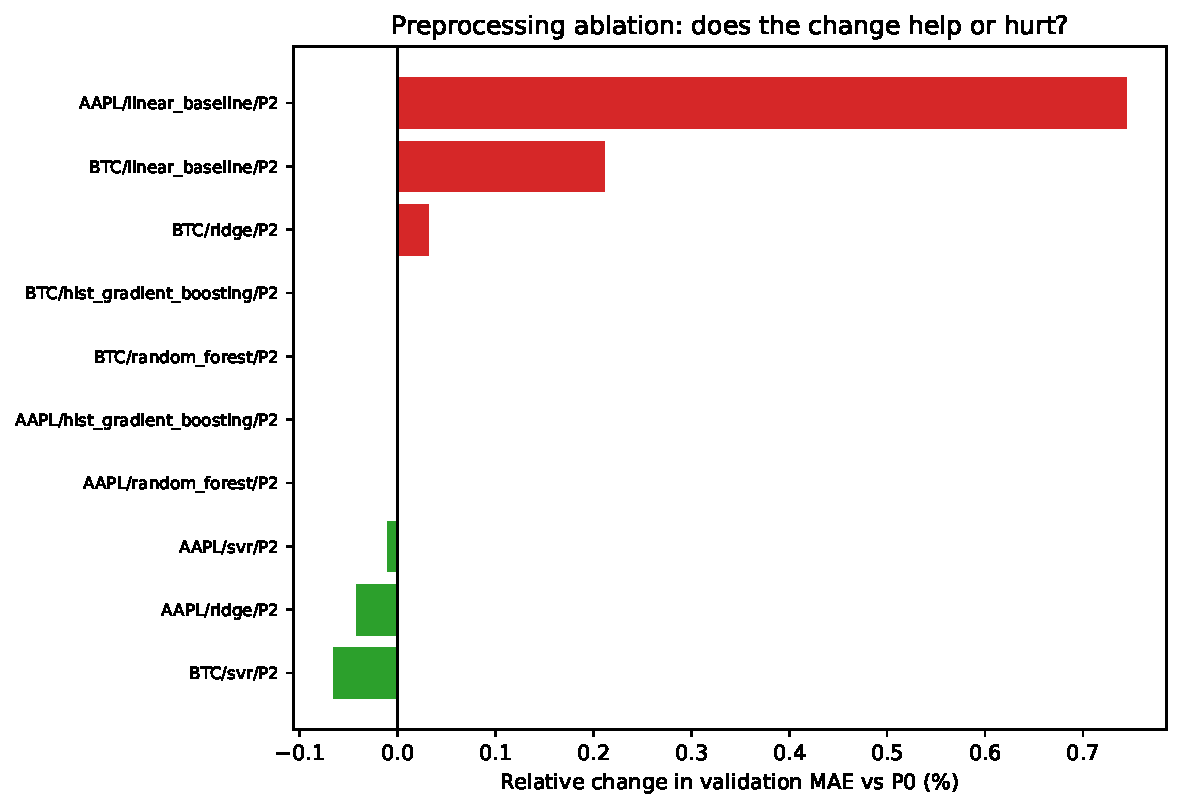
\includegraphics[width=\linewidth]{figures/fig06_ablation_delta.pdf}
  \caption{Relative change in validation MAE between unscaled (P0) and
  standardised (P2) variants, holding model and asset fixed. Bars at exactly zero
  are the tree ensembles, whose predictions are bit-identical under monotone
  rescaling. Only matched cells are plotted.}
  \label{fig:ablation}
\end{figure}

\section{Evaluation and Results}
\label{sec:results}

Table~\ref{tab:results} reports validation performance; all \NRunTotal{} runs
completed successfully and none read the test block.

\input{generated/results_table}

\paragraph{RQ1: nothing meaningfully beats persistence.}
The best result is \BestAAPLModel{} on AAPL at \BestAAPLSkill\% skill and
\BestBTCModel{} on BTC at \BestBTCSkill\% --- a fraction of a percentage point
above doing nothing. Two models are worse: the random forest on AAPL
(\SkillAAPLRandomForest\%) and the boosted ensemble on BTC
(\SkillBTCHistGradientBoosting\%).
\begin{figure}[t]
  \centering
  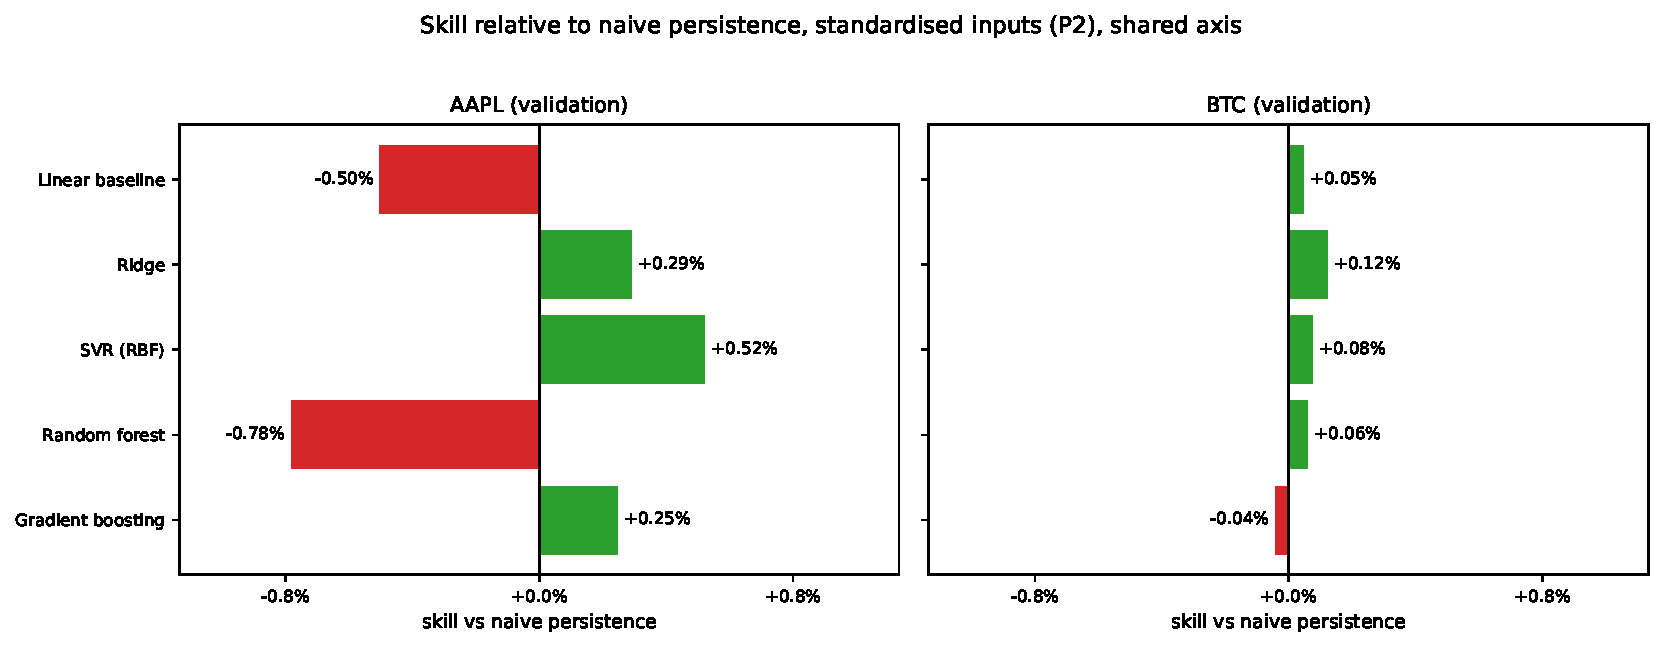
\includegraphics[width=\linewidth]{figures/fig04_model_vs_naive.pdf}
  \caption{Skill relative to naive persistence, per asset, on a \emph{shared}
  horizontal axis. Sharing matters: per-panel autoscaling would make BTC's
  fraction of a percent look as large as AAPL's. Bars left of zero are worse than
  repeating the current price.}
  \label{fig:skill}
\end{figure}

\paragraph{RQ2: capacity and regimes.}
Figure~\ref{fig:assets} gives the mechanical explanation: BTC's volatility is
higher and more variable, so a model with capacity fixed by an identical budget
faces a harder target, and every BTC skill value is closer to zero. On AAPL, where
capacity has more room to matter, the most flexible ensemble does worst --- the
signature of fitting noise.

\begin{figure}[t]
  \centering
  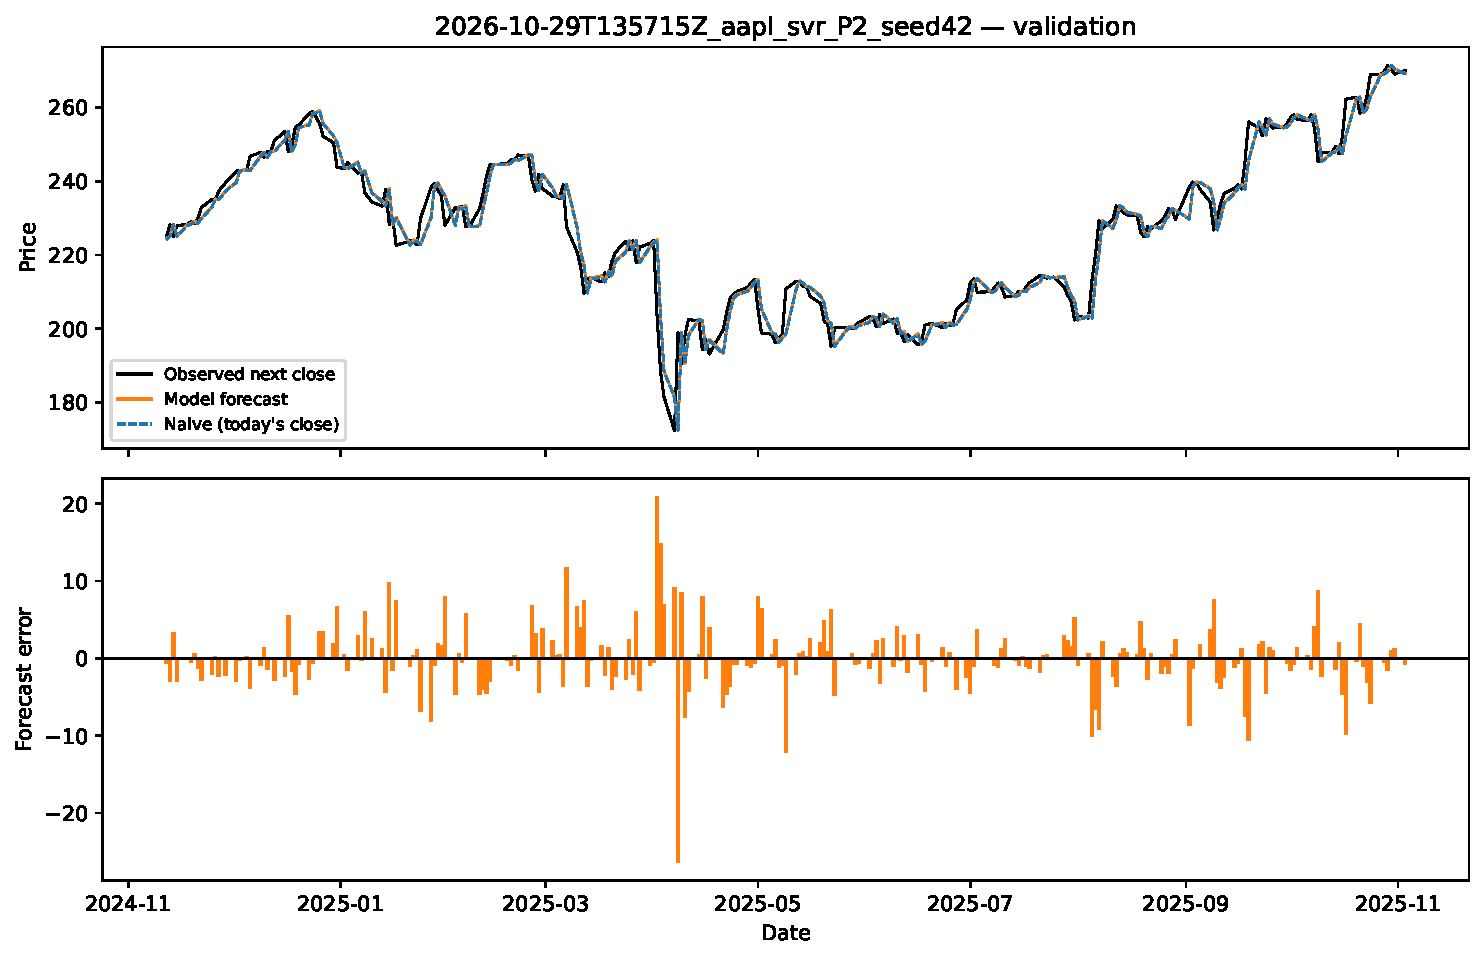
\includegraphics[width=0.78\linewidth]{figures/fig03_observed_vs_predicted_2026-10-29T135715Z_aapl_svr_P2_seed42_validation.pdf}
  \caption{Observed next close against the fitted SVR and naive forecasts on the
  AAPL validation block, with signed error below. The naive line tracks the
  observed series closely, which is why absolute error is a poor way to judge a
  model and skill is used instead.}
  \label{fig:forecast}
\end{figure}

\paragraph{Why they fail.}
The explanation is statistical, not architectural: daily return autocorrelation is
close to zero, so the features carry little information about the next session's
direction and extra parameters fit noise. The forest adds a structural limit ---
its predictions average leaf values, so it cannot extrapolate. Since all skill values lie within about one percentage point and the middle
ranking changes between assets, we claim no family is superior: the conclusion is
a tie against the baseline.

\begin{figure}[t]
  \centering
  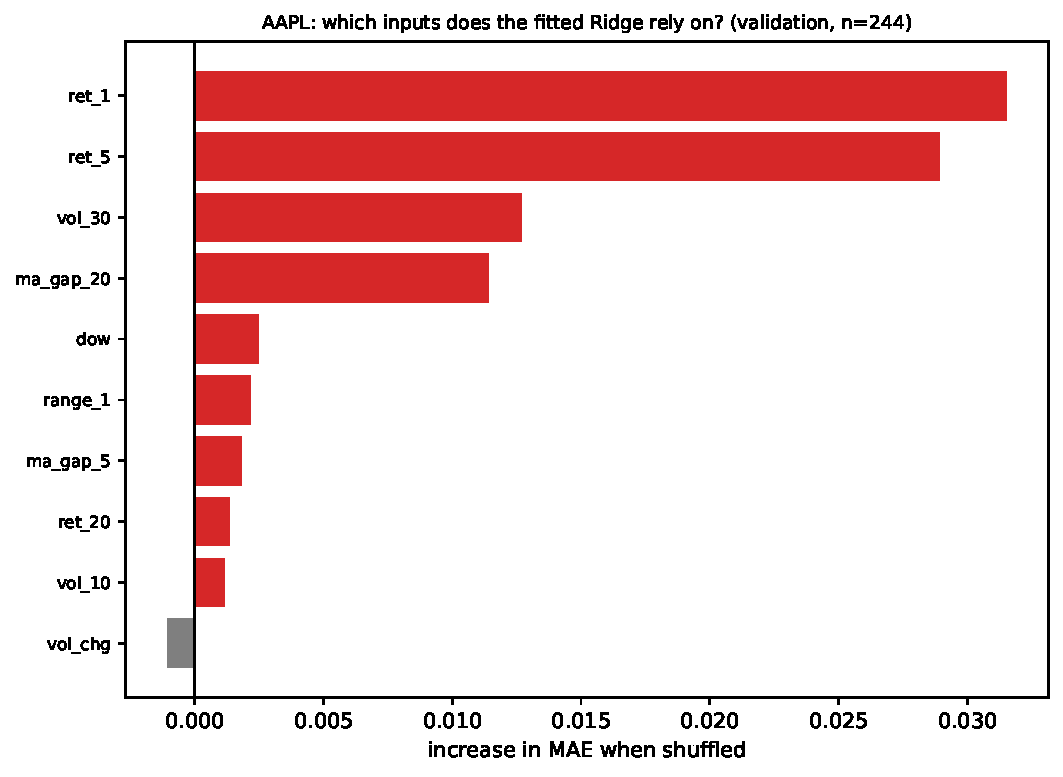
\includegraphics[width=0.76\linewidth]{figures/fig07_feature_importance_aapl.pdf}
  \caption{Learner-facing interpretability: permutation importance for the fitted
  Ridge model on the AAPL validation block, measured as the increase in MAE when
  one feature is shuffled \citep{fisher2019allmodels}. The model relies most on short-horizon returns and
  trailing volatility, and the magnitudes are tiny --- consistent with the skill
  table. This describes the fitted model, not a causal claim about markets.}
  \label{fig:importance}
\end{figure}

\section{Neural Networks (Experimental)}
\label{sec:dl}

Outside the main protocol, an MLP on the ten features and an LSTM on their last 20
days \repofile{scripts/supplementary_direction_test.py}{predicted next-day
direction}. We tuned them on the end of the training block and averaged over
\SupSeeds{} seeds (Table~\ref{tab:dl}). Training used Adam, batch size 64 and at
most \SupMaxEpochs{} epochs, with patience \SupPatience.

\begin{itemize}
  \item \textbf{AAPL:} both scored below ``always up''.
  \item \textbf{BTC:} both scored above ``always down'', but \textbf{all \SupNCi{}
  intervals include zero}.
  \item Hold-out log-loss (\SupLossLo--\SupLossHi) is close to the coin-flip value
  $\ln 2 \approx 0.693$.
\end{itemize}

\textbf{No clear evidence that these networks add predictive signal.}

\input{generated/dl_table}

\section{Educational Implications}
\label{sec:education}

RQ4 asks what these results can teach; the answer is a designed resource, not a
measured outcome. No learners were observed or surveyed, so these statements describe what a lesson
makes visible, not what anyone learned.

The lesson has five observable objectives: explain why a model that scores well
historically may fail tomorrow; identify leakage in a code fragment; interpret a
skill score including a negative one; predict which families are scale-sensitive
and justify it mechanistically; and distinguish forecast error from profitability.
Each is anchored to a real artefact: the negative random-forest entry in
Table~\ref{tab:results} is the teaching moment for the third, and
Figure~\ref{fig:ablation} asks why the tree bars are exactly zero.

Its most valuable property is that the headline result is negative. A demonstration
where the sophisticated model wins teaches that complexity is good; this one
teaches the transferable question \emph{what is the baseline, and did we beat it?}
Five formative tasks with worked answers accompany it, and the notebook lets a
non-specialist re-run the comparison.

\section{Limitations and Threats to Validity}
\label{sec:limitations}

\paragraph{Scope and target.}
Two assets, one window, one horizon, one convention. BTC is a single venue's USDT
price, not a global index. The label is the raw close one session ahead, so
dividends are ignored, and a one-session horizon is where persistence is
strongest --- a bias against trained models that follows from the question we
chose, and the reason H1 was pre-registered rather than discovered.

\paragraph{Statistics and evaluation integrity.}
Skill differences are within about one percentage point and intervals overlap, so
we report a tie; because errors are serially dependent, even block resampling
understates uncertainty. Every number here is a validation number, and validation
influenced model selection, so it is not a clean holdout; the sealed block exists
to give one unbiased estimate once the analysis is frozen.

\paragraph{Measurement integrity.}
Two leakage defects were found by independent audit and fixed. Both would have inflated results, and both were invisible to the authors of the
code: the audit mechanism, not the initial implementation, is what makes these
numbers trustworthy.

\paragraph{Education.}
No learner study was run, so claims about the lesson are design claims.

\section{Challenges and Team Learnings}
\label{sec:learnings}

The first challenge was target representation. Initial runs reported skill near
$-1800\%$. The features contained no price level, so the models could not recover
it and collapsed towards the training mean. After seeing this, we changed the
training target to the price change and recorded the decision.

The second was the boundary purge, found when an auditor traced a label to a test
price. Our first leakage tests had also passed with a one-bar forward shift
present. A passing test suite means more once it has been shown able to fail.

The third was fairness. Sharing one construction path, tuning budget and feature
set took more effort than fitting the models, but it made the comparison
meaningful.

\section{Conclusion}
\label{sec:conclusion}

Under a documented, leakage-audited protocol, none of five models meaningfully or
consistently outperformed a one-line persistence rule at predicting the next close
of Apple and Bitcoin. The best skill was \BestAAPLSkill\%, \NBelowAll{} of
\NRunTotal{} runs were worse than the rule, and the experimental networks showed no
clear advantage on direction.

For this course, the negative result supports the main lesson: ask of any model
what it beat, and how you know. The repository lets readers check the claim.
Nothing here is investment advice, and we have not measured learning gains.




\section*{Acknowledgements}
\addcontentsline{toc}{section}{Acknowledgements}
\noindent The repository holds hashed data snapshots, the protocol, run manifests,
tests and the notebook. AI coding assistants (Pi with
\texttt{pi-subagents}, and Claude Code) drafted code, tests and text under a
documented protocol. Zhang Yancheng directed that work: he
set the research direction, made the final decisions, and reviewed and verified
every AI-assisted change. This work is
educational, not investment advice.

\bibliographystyle{plainnat}
\bibliography{references}

\end{document}
"
% ---------------------------------------------------------------------------
\providecommand{\GroupAuthors}{%
  Zhang Yancheng \quad Dong Yuankun \quad Zhang Haoyu \\
  Lau Pak Hei \quad Lui Shing Lam}

% GENERATED by scripts/build_latex_assets.py -- do not edit by hand.
% Measured values referenced from prose, so no number is retyped by hand.
\newcommand{\NRunTotal}{20}
\newcommand{\NValAAPL}{244}
\newcommand{\BestAAPLModel}{SVR (RBF)}
\newcommand{\BestBTCModel}{Ridge}
\newcommand{\BestAAPLSkill}{+0.52}
\newcommand{\BestBTCSkill}{+0.12}
\newcommand{\SkillAAPLLinearBaseline}{-0.50}
\newcommand{\MaeAAPLLinearBaseline}{2.92}
\newcommand{\SkillAAPLRidge}{+0.29}
\newcommand{\MaeAAPLRidge}{2.90}
\newcommand{\SkillAAPLSvr}{+0.52}
\newcommand{\MaeAAPLSvr}{2.89}
\newcommand{\SkillAAPLRandomForest}{-0.78}
\newcommand{\MaeAAPLRandomForest}{2.93}
\newcommand{\SkillAAPLHistGradientBoosting}{+0.25}
\newcommand{\MaeAAPLHistGradientBoosting}{2.90}
\newcommand{\SkillBTCLinearBaseline}{+0.05}
\newcommand{\MaeBTCLinearBaseline}{1603.59}
\newcommand{\SkillBTCRidge}{+0.12}
\newcommand{\MaeBTCRidge}{1602.39}
\newcommand{\SkillBTCSvr}{+0.08}
\newcommand{\MaeBTCSvr}{1603.13}
\newcommand{\SkillBTCRandomForest}{+0.06}
\newcommand{\MaeBTCRandomForest}{1603.37}
\newcommand{\SkillBTCHistGradientBoosting}{-0.04}
\newcommand{\MaeBTCHistGradientBoosting}{1605.02}
\newcommand{\NBelowAll}{5}
\newcommand{\NBelowPtwo}{3}
\newcommand{\BestBTCAllModel}{Linear baseline}
\newcommand{\BestBTCAllVariant}{P0}
\newcommand{\BestBTCAllSkill}{+0.26}
\newcommand{\NValBTC}{358}
\newcommand{\TrialsUsed}{10}
\newcommand{\SecondsUsed}{90}
\newcommand{\TrialsMax}{24}
\newcommand{\SecondsMax}{300}
\newcommand{\NCiTotal}{20}
\newcommand{\NCiIncludeZero}{20}
\newcommand{\SupPresent}{yes}
\newcommand{\SupNCi}{4}
\newcommand{\SupNCiZero}{4}
\newcommand{\SupLossLo}{0.676}
\newcommand{\SupLossHi}{0.697}
\newcommand{\SupSeeds}{5}
\newcommand{\SupMaxEpochs}{300}
\newcommand{\SupPatience}{20}


\title{\vspace{-1.2cm}\bfseries Learning Machine Learning Through Financial
Time-Series Forecasting:\\[2pt]
\large A Reproducible Comparison of Models and Preprocessing Strategies on
Apple and Bitcoin}
\author{\GroupAuthors\\[2pt]
\small INT4096 Artificial Intelligence and Machine Learning in Education\\
\small The Education University of Hong Kong, Semester 1, 2026--27}
\date{28 November 2026}

\begin{document}
\maketitle
\vspace{-0.6cm}

\begin{abstract}
\noindent
Financial forecasting makes generalisation, leakage and baseline comparison
checkable. We compare five models and two preprocessing variants for next-session
close prediction on Apple (AAPL) and Bitcoin (BTC) under a documented,
leakage-audited protocol. Across \NRunTotal{} runs, no model beat naive persistence
by more than \BestAAPLSkill\% (AAPL) or \BestBTCAllSkill\% (BTC), \NBelowAll{} runs
were worse, and every bootstrap interval includes zero. Experimental neural
networks showed no clear advantage. We turn this negative result into a
five-objective lesson on reading skill scores, finding leakage and understanding
scaling. Without a learner study, we make no claim of learning gains.
\end{abstract}

\vspace{0.2cm}
\section{Introduction and Educational Motivation}
\label{sec:intro}

Introductory machine learning often uses problems where better models visibly win.
Such examples can hide two questions that decide whether a model is useful:
\textbf{\emph{what did it learn}, and \emph{against what baseline}?}

Short-horizon prices are close to a random walk \citep{fama1970efficient}. A
sophisticated model can therefore lose to the rule \textbf{\emph{tomorrow's price
equals today's}}, and a learner who can explain why has understood more than a
leaderboard shows.

We compare two markets, Apple (AAPL) and Bitcoin (BTC). Our \textbf{audience} is
advanced secondary-school students, pre-university learners interested in AI, and
university students without a machine-learning major. The intended outcomes are
conceptual (Section~\ref{sec:education}).

\section{Theoretical Background}
\label{sec:background}

\paragraph{Regression and generalisation.}
We predict the close of session $t+1$ from features known at the close of session
$t$. Training error usually falls as capacity grows, so performance must be judged
on unseen data \citep{hastie2009elements}.

\paragraph{Model families.}
Ridge regression is a regularised linear model. Support vector regression with an
RBF kernel \citep{drucker1997support} predicts from weighted kernel similarities,
so it depends on distances in feature space. A random forest
\citep{breiman2001random} averages bootstrapped trees to reduce variance.
Histogram gradient boosting \citep{friedman2001gradient} fits trees sequentially
to residuals and can also fit noise.

\paragraph{Preprocessing is part of the model.}
A tree splits on $x_j < \tau$. Rescaling $x_j$ by a positive constant preserves
order, so an equivalent threshold exists. A kernel method sums squared differences
\emph{across} features, so rescaling changes which feature dominates. We test this
asymmetry in Section~\ref{sec:ablation}.

\paragraph{Ordered data and leakage.}
Random cross-validation lets a model interpolate across time and is invalid here
\citep{bergmeir2018note,roberts2017crossvalidation}. We use chronological splits
with a boundary purge. Leakage, meaning information unavailable at prediction
time, can make an evaluation optimistic \citep{kaufman2012leakage}, so we test for
it.

\section{Research Questions}
\label{sec:questions}

\begin{description}[leftmargin=1.4em,style=nextline]
  \item[RQ1.] Under identical, leakage-safe conditions, how do distinct model
  families perform against naive persistence on AAPL and BTC?
  \item[RQ2.] How do complexity, tuning and changing market conditions affect
  generalisation and error patterns?
  \item[RQ3.] To what extent do preprocessing and feature choices change forecast
  error, and does the effect depend on model family and market?
  \item[RQ4.] What do selected examples and counterexamples teach learners about
  model behaviour, evaluation and responsible interpretation?
\end{description}

Five hypotheses were fixed before any result was inspected: persistence is
competitive at this horizon (H1); AAPL is more predictable than BTC (H2); scaling
moves error more for scaling-sensitive families than for trees (H3); complexity
widens the train--validation gap (H4); features matter more than the scaler (H5).
RQ4 is answered by an artefact, not a learner study, and H1 turning out true is an
acceptable outcome.

\section{Dataset and Data Provenance}
\label{sec:data}

\textbf{Two public datasets, saved once and never edited.} Each experiment
\textbf{re-checks the SHA-256 fingerprint} and stops on a mismatch
(\repodir{data/raw}{raw data}, \repodir{data/cards}{dataset cards}).

\begin{table}[H]
\centering
\caption{Where the data came from and how many rows we use. Modelling rows exclude
the first \Warmup{} bars (feature windows not yet full) and the last bar (no next
close).}
\label{tab:dataset}
\small
\begin{tabular}{@{}L{0.20\linewidth} L{0.36\linewidth} L{0.36\linewidth}@{}}
\toprule
 & \textbf{Apple (AAPL)} & \textbf{Bitcoin (BTC/USDT)} \\
\midrule
\textbf{Source} & StockAnalysis public history API & Binance public REST API, spot \\
Endpoint & \scriptsize\url{https://stockanalysis.com/api/symbol/s/aapl/history} & \scriptsize\url{https://api.binance.com/api/v3/klines} \\
Fields & date, open, high, low, close, volume, adjusted close & open time, open, high, low, close, volume \\
\textbf{Window} & \WindowAAPL & \WindowBTC \\
Daily bars & \ObsAAPL & \ObsBTC \\
Quality checks$^{*}$ & \textbf{\QualityAAPL} & \textbf{\QualityBTC} \\
\textbf{Modelling rows} & \textbf{\RowsAAPL} & \textbf{\RowsBTC} \\
Train / validation / test & \TrainRowsAAPL{} / \ValidationRowsAAPL{} / \TestRowsAAPL & \TrainRowsBTC{} / \ValidationRowsBTC{} / \TestRowsBTC \\
\bottomrule
\end{tabular}
\par\smallskip\footnotesize
$^{*}$Duplicate dates, missing values, non-positive prices, inconsistent high, low or close, negative volume.
\end{table}

\begin{table}[H]
\centering
\caption{The two datasets differ. How we handled each difference.}
\label{tab:differences}
\small
\begin{tabular}{@{}L{0.16\linewidth} L{0.21\linewidth} L{0.19\linewidth} L{0.35\linewidth}@{}}
\toprule
Difference & AAPL & BTC & \textbf{What we did} \\
\midrule
Unit & listed share, USD & one exchange, USDT & Compare assets only by \textbf{unit-free skill} \\
Calendar & exchange sessions; \GapsAAPL{} weekend or holiday gaps & every day & Keep \textbf{each calendar}; never align rows \\
Close range & \CloseRangeAAPL & \CloseRangeBTC & Use \textbf{returns and ratios} as inputs \\
Daily volatility & \RetSdAAPL\% & \RetSdBTC\% & \textbf{Fit and score separately} \\
Adjusted price & differs on \AdjDiffPctAAPL\% of days & none & Predict the \textbf{raw close} \\
\bottomrule
\end{tabular}
\end{table}

Providers revise adjusted prices later, so they contain \textbf{information
unavailable at decision time}. No split discontinuity falls in the window (the
adjusted/raw ratio never jumps by more than 2\%), and we ignore dividends.

% Keep the generated split table here, in numbering order.
\begingroup
\let\floatingtable\table
\renewcommand{\table}[1][]{\floatingtable[H]}
% GENERATED by scripts/build_latex_assets.py -- do not edit by hand.
\begin{table}[t]
\centering
\caption{Chronological split boundaries in the asset's own calendar. One row is purged at each boundary so that no label crosses a split: with $y_t = C_{t+1}$, the last training label would otherwise be a validation price and the last validation label a sealed test price. The test block remains unopened.}
\label{tab:splits}
\small
\setlength{\tabcolsep}{4pt}
\begin{tabular}{@{}l l l l r@{}}
\toprule
Asset & Training & Validation & Sealed test & Total \\
\midrule
AAPL & 2021-12-10..2024-11-08 & 2024-11-12..2025-11-03 & 2025-11-05..2026-10-27 & 1,224 \\
BTC & 2021-11-27..2024-11-07 & 2024-11-09..2025-11-01 & 2025-11-03..2026-10-28 & 1,797 \\
\bottomrule
\end{tabular}
\par\smallskip\footnotesize
Total is the number of usable feature rows after the trailing-window warm-up and the terminal unlabelled row are removed.
\end{table}

\endgroup

\begin{figure}[t]
  \centering
  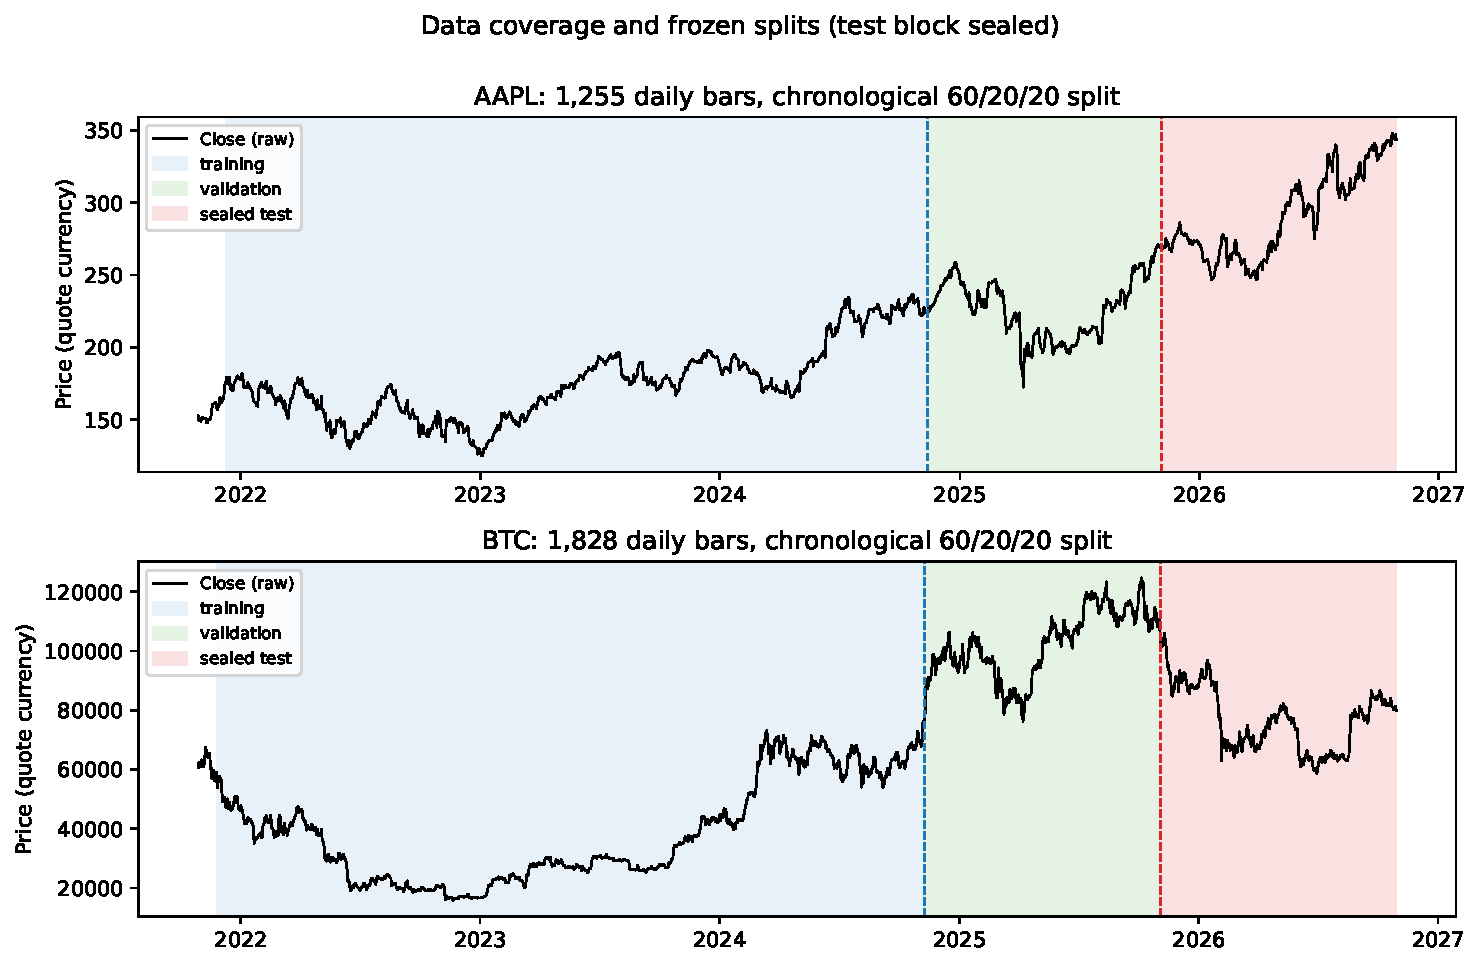
\includegraphics[width=0.9\linewidth]{figures/fig01_coverage_and_splits.pdf}
  \caption{Price history with the fixed 60/20/20 chronological split. Blue is
  training, green validation, red the \textbf{sealed test block}, which no run has
  read. The unshaded start is the feature warm-up.}
  \label{fig:coverage}
\end{figure}

\begin{figure}[t]
  \centering
  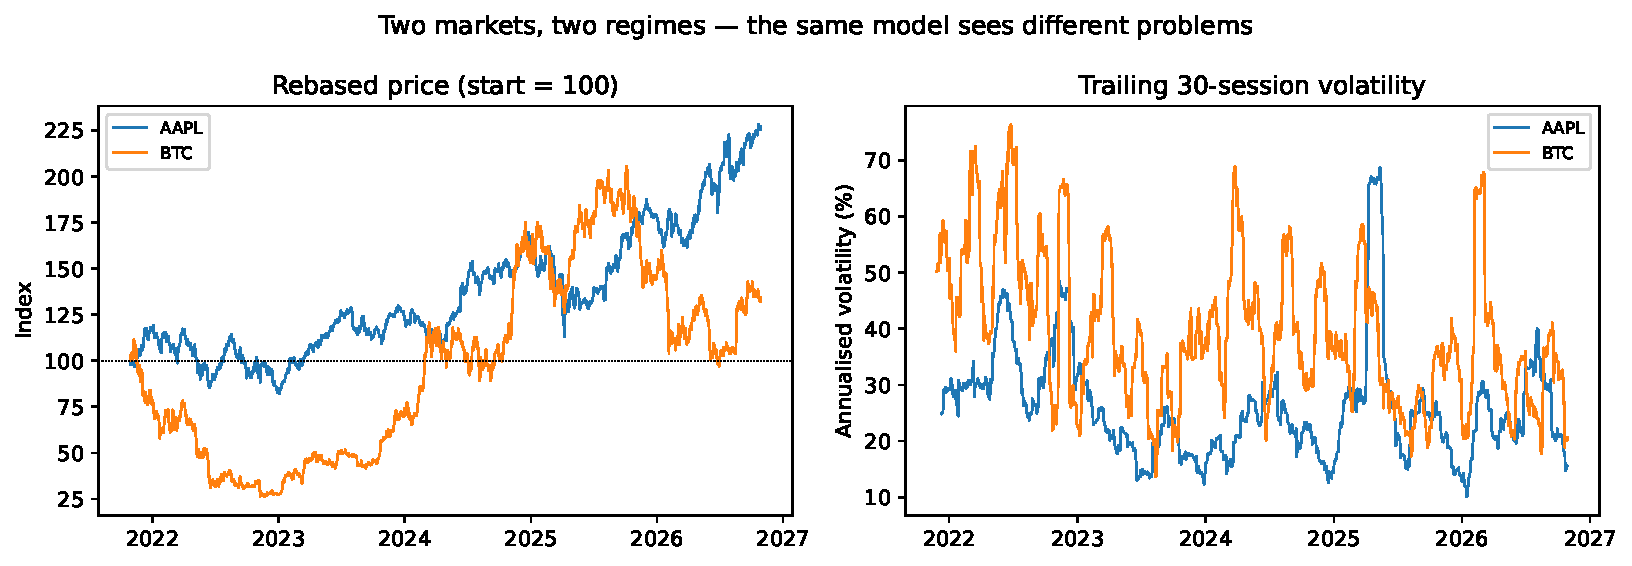
\includegraphics[width=0.9\linewidth]{figures/fig02_asset_characteristics.pdf}
  \caption{How the markets differ. Left: each series rebased to 100. Right:
  annualised 30-session volatility. BTC is usually more volatile.}
  \label{fig:assets}
\end{figure}

\section{Features and Leakage Control}
\label{sec:features}

The ten features are trailing ratios: returns over 1, 5 and 20 sessions; gaps to
5- and 20-session moving averages; realised volatility over 10 and 30 sessions;
intra-bar range; a volume anomaly; and day of week. Each uses bars up to and
including $t$, and rolling statistics require a full window.

Features are \emph{scale free} rather than price levels, which are non-stationary
and would let a model look accurate by copying today's price. The
reported quantity is error on the next close \emph{price}, while models are fitted
on the price \emph{change} and reconstructed as
$\hat{C}_{t+1} = C_t + \widehat{\Delta}_t$. The two are information-equivalent
because $C_t$ is known at decision time.

\paragraph{Boundary purge.}
With $y_t = C_{t+1}$, the last training label is a validation price and the last
validation label a sealed test price, so one row is dropped at each boundary. An
independent audit showed that, without it, perturbing one test price moved the
headline metric by 0.408 (Table~\ref{tab:splits}).

% GENERATED by scripts/build_latex_assets.py -- do not edit by hand.
\begin{table}[t]
\centering
\caption{Chronological split boundaries in the asset's own calendar. One row is purged at each boundary so that no label crosses a split: with $y_t = C_{t+1}$, the last training label would otherwise be a validation price and the last validation label a sealed test price. The test block remains unopened.}
\label{tab:splits}
\small
\setlength{\tabcolsep}{4pt}
\begin{tabular}{@{}l l l l r@{}}
\toprule
Asset & Training & Validation & Sealed test & Total \\
\midrule
AAPL & 2021-12-10..2024-11-08 & 2024-11-12..2025-11-03 & 2025-11-05..2026-10-27 & 1,224 \\
BTC & 2021-11-27..2024-11-07 & 2024-11-09..2025-11-01 & 2025-11-03..2026-10-28 & 1,797 \\
\bottomrule
\end{tabular}
\par\smallskip\footnotesize
Total is the number of usable feature rows after the trailing-window warm-up and the terminal unlabelled row are removed.
\end{table}


\paragraph{Enforcement.}
One test recomputes every feature from raw data with trailing formulas written
separately in the test, so a forward peek mismatches; another appends absurd future
prices and asserts earlier values are unchanged. Six canonical defects --- a
one-bar forward shift, an obfuscated equivalent, a centred window, a backward
fill, a whole-series statistic, and preprocessing fitted on train-plus-test ---
are then injected one at a time, and each must be detected.

\section{Experimental Methodology}
\label{sec:method}

Each asset is split chronologically into 60\% training, 20\% validation and 20\%
sealed test on its own session index, with a one-row purge at each boundary
(Table~\ref{tab:splits}); all models see identical boundaries and dates. Hyperparameters are chosen by random search inside an
expanding-window time-series cross-validation confined to the training block:
five folds, a one-fold gap, minimum initial training fraction 0.30. Because
tuning never sees validation, validation remains a selection holdout rather than
a second tuning set. Every family gets the same budget, \TrialsUsed{} trials and at most \SecondsUsed{}~s
per cell (the protocol caps \TrialsMax{} and \SecondsMax{}~s), and every attempted
configuration is logged.

\begin{figure}[t]
  \centering
  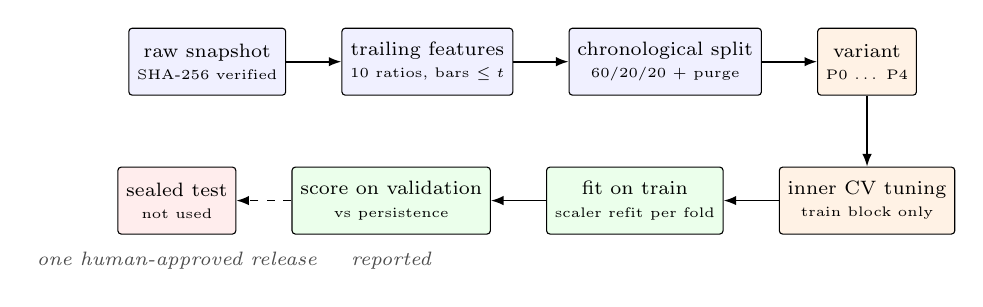
\begin{tikzpicture}[
      node distance=5mm and 7mm,
      box/.style={draw, rounded corners=1.2pt, align=center, font=\scriptsize,
                  inner sep=3pt, minimum height=8.5mm},
      arr/.style={-{Latex[length=1.6mm]}, semithick},
      lbl/.style={font=\scriptsize\itshape, text=black!70}]
    \node[box, fill=blue!6] (raw) {raw snapshot\\{\tiny SHA-256 verified}};
    \node[box, fill=blue!6, right=of raw] (feat) {trailing features\\{\tiny 10 ratios, bars $\le t$}};
    \node[box, fill=blue!6, right=of feat] (split) {chronological split\\{\tiny 60/20/20 + purge}};
    \node[box, fill=orange!10, right=of split] (pre) {variant\\{\tiny P0 \dots\ P4}};
    \node[box, fill=orange!10, below=9mm of pre] (tune) {inner CV tuning\\{\tiny train block only}};
    \node[box, fill=green!8, left=of tune] (fit) {fit on train\\{\tiny scaler refit per fold}};
    \node[box, fill=green!8, left=of fit] (eval) {score on validation\\{\tiny vs persistence}};
    \node[box, fill=red!7, left=of eval] (test) {sealed test\\{\tiny not used}};

    \draw[arr] (raw) -- (feat);
    \draw[arr] (feat) -- (split);
    \draw[arr] (split) -- (pre);
    \draw[arr] (pre) -- (tune);
    \draw[arr] (tune) -- (fit);
    \draw[arr] (fit) -- (eval);
    \draw[arr, dashed] (eval) -- (test);
    \node[lbl, below=1mm of eval] {reported};
    \node[lbl, below=1mm of test] {one human-approved release};
  \end{tikzpicture}
  \caption{The experiment pipeline, drawn to match the implementation. The scaler
  is fitted \emph{inside} the model pipeline, so it is refitted per fold and
  cannot see validation rows. Dashed arrow: the test block is not evaluated by
  any run in this report.}
  \label{fig:pipeline}
\end{figure}

We report MAE, RMSE and $R^2$, plus \emph{skill} relative to persistence on
identical forecast dates:
\begin{equation*}
  \text{skill}_{\text{MAE}} \;=\; 1 - \frac{\text{MAE}_{\text{model}}}{\text{MAE}_{\text{naive}}}.
\end{equation*}
Skill is primary because it has a meaningful zero. $R^2$ is inflated on a trending level: our naive forecast itself attains $R^2 \approx 0.96$, so a high $R^2$
here indicates a trending series, not a good model. Absolute errors are never
compared across assets. Uncertainty uses a moving-block bootstrap over consecutive dates; overlapping blocks retain dependence, so we treat it as indicative only.

\section{Model Selection and Baselines}
\label{sec:models}

The five families differ in mechanism rather than to reach a count: a
near-unregularised linear model as a learned floor, Ridge as a regularised linear
reference, RBF support vector regression as a kernel method, a random forest as a
bagged ensemble, and histogram gradient boosting as a boosted ensemble. A shallow neural network was considered and left gated: the written handout
discourages deep learning, and the instructor's reported oral guidance is recorded
as reported guidance, not as a changed rule, so that lane does not appear here.

The mandatory baseline is naive persistence, $\hat{C}_{t+1} = C_t$. It is not a straw man: for a near-random-walk series it is strong, free, and
defines the zero of the skill scale \citep{makridakis2018m4,hyndman2021fpp3}. Forecasting competitions reach the same conclusion
about simple benchmarks \citep{makridakis2018m4,hyndman2021fpp3}.

Every family is built through one shared code path, so each receives identical
feature columns in identical order and any scaler sits inside its pipeline where
it is refitted per fold. Tests assert that column identity and that a fixed seed
is deterministic.

\section{Preprocessing Ablation}
\label{sec:ablation}

RQ3 asks how much preprocessing matters. We vary one factor at a time, holding
model, features, split and tuning budget fixed; the contrast is scaling, with P0
unscaled and P2 standardised on training rows only.

% GENERATED by scripts/build_latex_assets.py -- do not edit by hand.
\begin{table}[t]
\centering
\caption{Controlled preprocessing ablation: validation MAE without standardisation (P0) and with it (P2), holding model, features, split and tuning budget fixed. A change of exactly $0.000\%$ means the model is invariant to monotone per-feature rescaling, which is the theoretical prediction for tree ensembles and serves as a negative control.}
\label{tab:ablation}
\small
\setlength{\tabcolsep}{4pt}
\begin{tabular}{@{}l r r r r r@{}}
\toprule
 & \multicolumn{3}{c}{AAPL} & \multicolumn{2}{c}{BTC} \\
\cmidrule(lr){2-4}\cmidrule(l){5-6}
Model & P0 MAE & P2 MAE & $\Delta$ & P0 MAE & $\Delta$ \\
\midrule
Linear baseline & 2.899 & 2.920 & +0.745 & 1600.205 & +0.211 \\
Ridge & 2.898 & 2.897 & -0.041 & 1601.874 & +0.032 \\
SVR (RBF) & 2.891 & 2.890 & -0.010 & 1604.186 & -0.066 \\
Random forest & 2.928 & 2.928 & \textbf{0.000} & 1603.373 & \textbf{0.000} \\
Hist.\ gradient boosting & 2.898 & 2.898 & \textbf{0.000} & 1605.016 & \textbf{0.000} \\
\bottomrule
\end{tabular}
\par\smallskip\footnotesize
$\Delta$ is the percentage change in validation MAE from P0 to P2. Bold $0.000$ denotes bit-identical predictions.
\end{table}


The measured pattern matches Section~\ref{sec:background}, exactly rather than
approximately: for both tree ensembles the change in validation MAE is
\emph{bit-identical} --- $0.000\%$ to printed precision --- on both assets. That is a strong internal control: had scaling moved the forests, the correct
inference would be a bug, not a discovery.

Scaling-sensitive families move slightly and not uniformly helpfully:
standardisation barely changes AAPL Ridge, worsens the AAPL linear baseline
(Table~\ref{tab:ablation}) and rescues nothing --- every value stays within about
one percentage point of the baseline. An ablation ending in no
substantial effect is a legitimate finding, and a useful teaching one: it
separates \emph{this transform changes the model} from \emph{this transform
improves the forecast}.

One variant is reported as not run: with no missing values in either snapshot an
imputation variant would duplicate the baseline cell, and we did not inject
synthetic gaps to manufacture a contrast.

\begin{figure}[t]
  \centering
  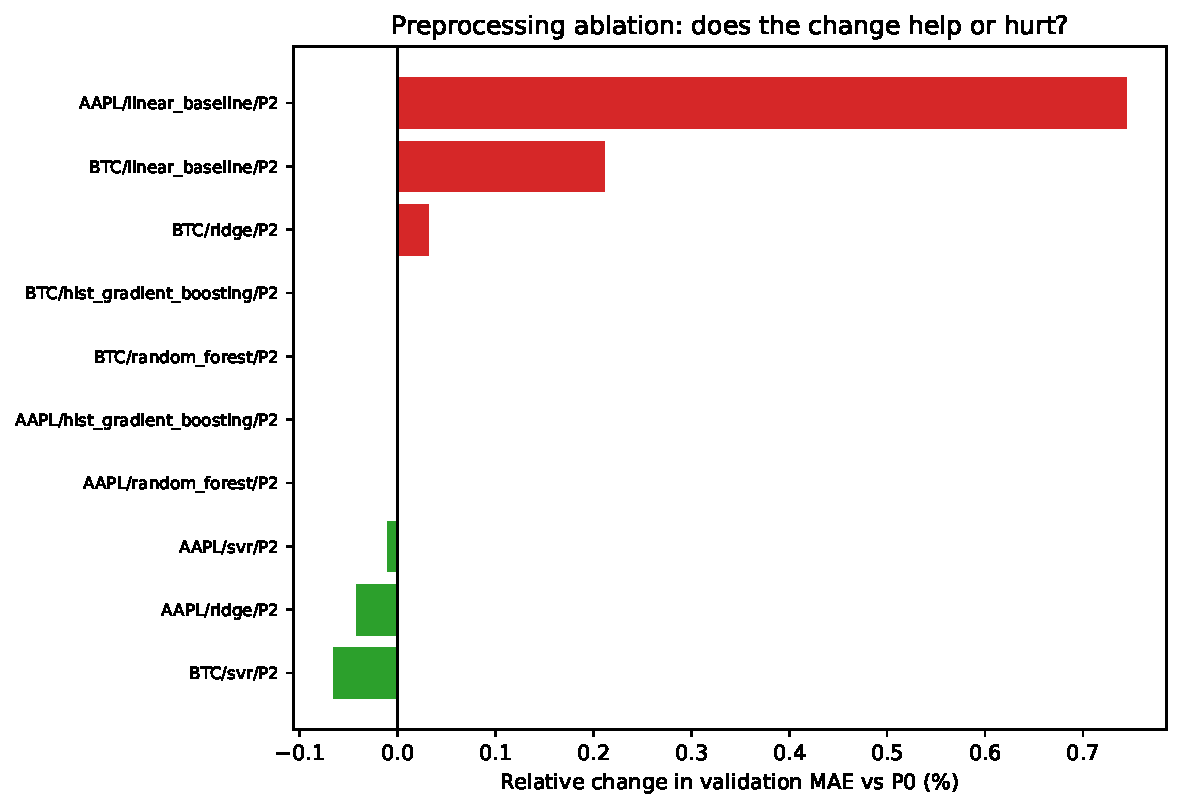
\includegraphics[width=\linewidth]{figures/fig06_ablation_delta.pdf}
  \caption{Relative change in validation MAE between unscaled (P0) and
  standardised (P2) variants, holding model and asset fixed. Bars at exactly zero
  are the tree ensembles, whose predictions are bit-identical under monotone
  rescaling. Only matched cells are plotted.}
  \label{fig:ablation}
\end{figure}

\section{Evaluation and Results}
\label{sec:results}

Table~\ref{tab:results} reports validation performance; all \NRunTotal{} runs
completed successfully and none read the test block.

% GENERATED by scripts/build_latex_assets.py -- do not edit by hand.
% Source: experiments/models/*/*/metrics.json (validation split only).
\begin{table}[t]
\centering
\caption{Validation performance for each model family under the shared protocol (variant P2, standardised inputs, seed 42). Skill is measured against naive persistence on identical forecast dates. Absolute errors are in quote currency and are \emph{not} comparable between AAPL and BTC; only the unitless skill column is. The test block was not used.}
\label{tab:results}
\small
\setlength{\tabcolsep}{4pt}
\begin{tabular}{@{}l r r r r r r@{}}
\toprule
 & \multicolumn{3}{c}{AAPL} & \multicolumn{3}{c}{BTC} \\
\cmidrule(lr){2-4}\cmidrule(l){5-7}
Model & MAE & RMSE & Skill & MAE & RMSE & Skill \\
\midrule
Linear baseline & 2.92 & 4.37 & \textbf{-0.50} & 1603.59 & 2211.24 & +0.05 \\
Ridge & 2.90 & 4.36 & +0.29 & 1602.39 & 2205.96 & +0.12 \\
SVR (RBF) & 2.89 & 4.36 & +0.52 & 1603.13 & 2203.85 & +0.08 \\
Random forest & 2.93 & 4.37 & \textbf{-0.78} & 1603.37 & 2208.04 & +0.06 \\
Hist.\ gradient boosting & 2.90 & 4.36 & +0.25 & 1605.02 & 2204.91 & \textbf{-0.04} \\
\midrule
Naive persistence & 2.91 & 4.36 & 0.00 & 1604.35 & 2205.67 & 0.00 \\
\bottomrule
\end{tabular}
\par\smallskip\footnotesize
Skill is $1 - \mathrm{MAE}_{\mathrm{model}}/\mathrm{MAE}_{\mathrm{naive}}$ in percent; negative values (bold) are worse than the baseline. $n=244$ (AAPL) and $358$ (BTC) validation sessions.
\end{table}


\paragraph{RQ1: nothing meaningfully beats persistence.}
The best result is \BestAAPLModel{} on AAPL at \BestAAPLSkill\% skill and
\BestBTCModel{} on BTC at \BestBTCSkill\% --- a fraction of a percentage point
above doing nothing. Two models are worse: the random forest on AAPL
(\SkillAAPLRandomForest\%) and the boosted ensemble on BTC
(\SkillBTCHistGradientBoosting\%).
\begin{figure}[t]
  \centering
  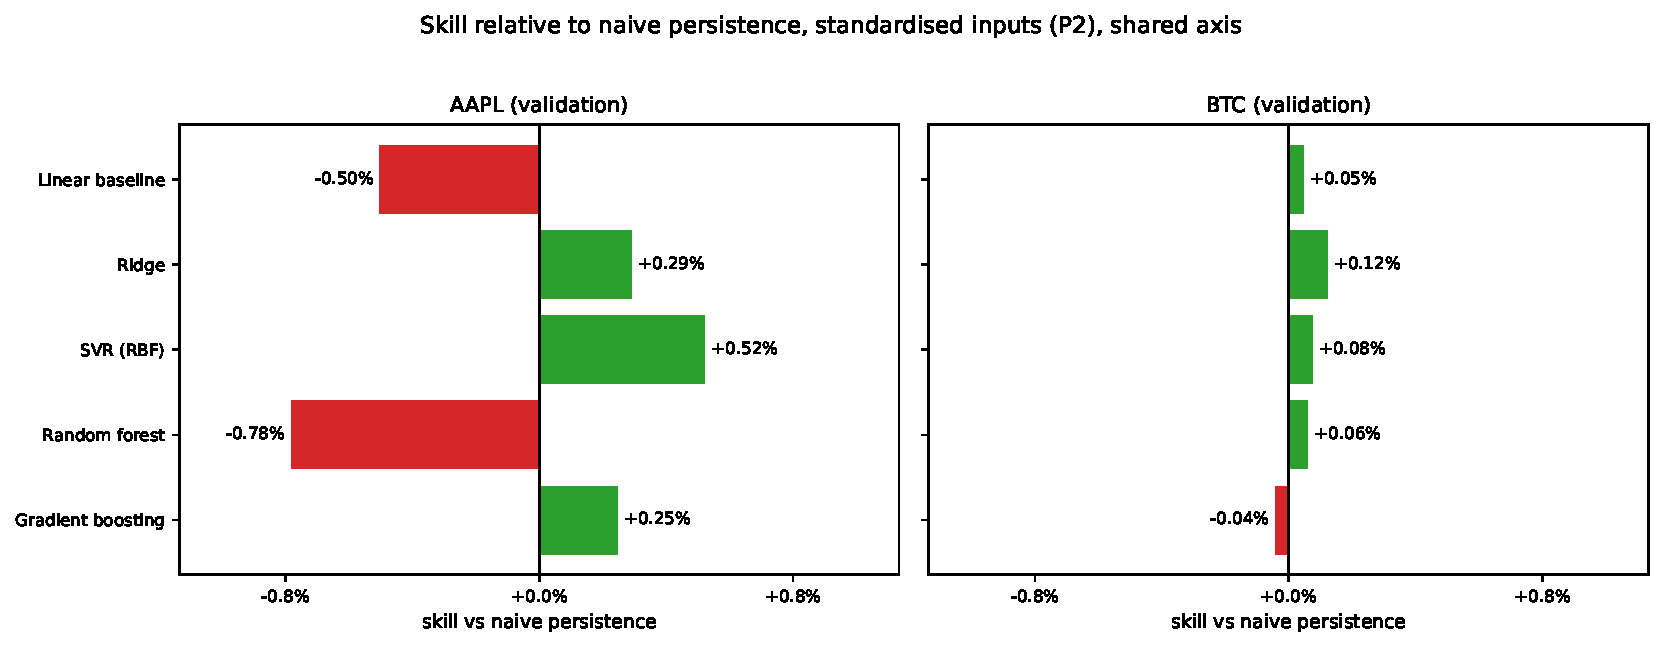
\includegraphics[width=\linewidth]{figures/fig04_model_vs_naive.pdf}
  \caption{Skill relative to naive persistence, per asset, on a \emph{shared}
  horizontal axis. Sharing matters: per-panel autoscaling would make BTC's
  fraction of a percent look as large as AAPL's. Bars left of zero are worse than
  repeating the current price.}
  \label{fig:skill}
\end{figure}

\paragraph{RQ2: capacity and regimes.}
Figure~\ref{fig:assets} gives the mechanical explanation: BTC's volatility is
higher and more variable, so a model with capacity fixed by an identical budget
faces a harder target, and every BTC skill value is closer to zero. On AAPL, where
capacity has more room to matter, the most flexible ensemble does worst --- the
signature of fitting noise.

\begin{figure}[t]
  \centering
  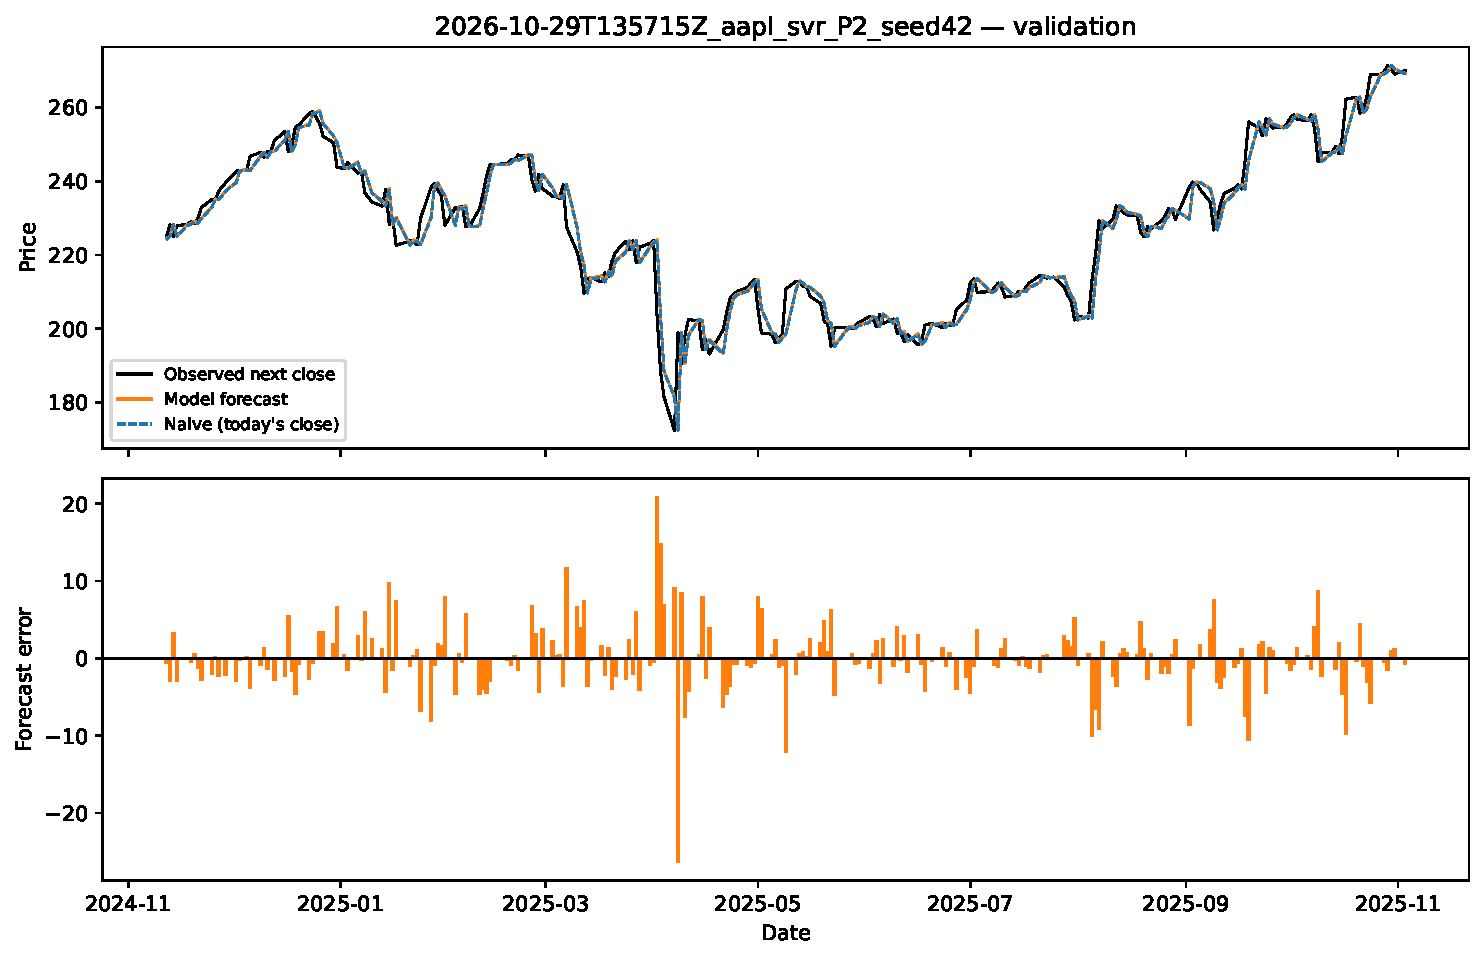
\includegraphics[width=0.78\linewidth]{figures/fig03_observed_vs_predicted_2026-10-29T135715Z_aapl_svr_P2_seed42_validation.pdf}
  \caption{Observed next close against the fitted SVR and naive forecasts on the
  AAPL validation block, with signed error below. The naive line tracks the
  observed series closely, which is why absolute error is a poor way to judge a
  model and skill is used instead.}
  \label{fig:forecast}
\end{figure}

\paragraph{Why they fail.}
The explanation is statistical, not architectural: daily return autocorrelation is
close to zero, so the features carry little information about the next session's
direction and extra parameters fit noise. The forest adds a structural limit ---
its predictions average leaf values, so it cannot extrapolate. Since all skill values lie within about one percentage point and the middle
ranking changes between assets, we claim no family is superior: the conclusion is
a tie against the baseline.

\begin{figure}[t]
  \centering
  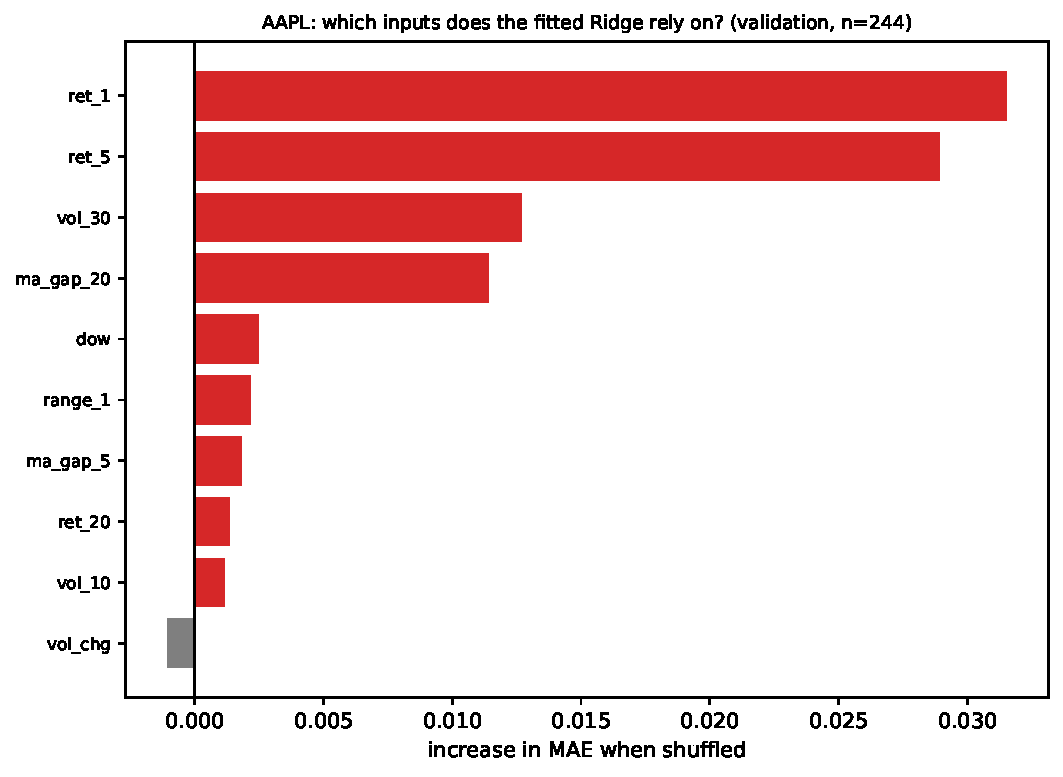
\includegraphics[width=0.76\linewidth]{figures/fig07_feature_importance_aapl.pdf}
  \caption{Learner-facing interpretability: permutation importance for the fitted
  Ridge model on the AAPL validation block, measured as the increase in MAE when
  one feature is shuffled \citep{fisher2019allmodels}. The model relies most on short-horizon returns and
  trailing volatility, and the magnitudes are tiny --- consistent with the skill
  table. This describes the fitted model, not a causal claim about markets.}
  \label{fig:importance}
\end{figure}

\section{Neural Networks (Experimental)}
\label{sec:dl}

Outside the main protocol, an MLP on the ten features and an LSTM on their last 20
days \repofile{scripts/supplementary_direction_test.py}{predicted next-day
direction}. We tuned them on the end of the training block and averaged over
\SupSeeds{} seeds (Table~\ref{tab:dl}). Training used Adam, batch size 64 and at
most \SupMaxEpochs{} epochs, with patience \SupPatience.

\begin{itemize}
  \item \textbf{AAPL:} both scored below ``always up''.
  \item \textbf{BTC:} both scored above ``always down'', but \textbf{all \SupNCi{}
  intervals include zero}.
  \item Hold-out log-loss (\SupLossLo--\SupLossHi) is close to the coin-flip value
  $\ln 2 \approx 0.693$.
\end{itemize}

\textbf{No clear evidence that these networks add predictive signal.}

% GENERATED by scripts/build_latex_assets.py -- do not edit by hand.
% Source: experiments/supplementary/direction_test/*/results.json (decision D14).
\begin{table}[t]
\centering
\caption{Experimental neural-network test: share of validation sessions whose next-day direction (up or not up) was called correctly. Seed range in brackets; interval = 95\% moving-block bootstrap of the difference from the majority rule, in percentage points. The LSTM reads a sequence, so its inputs differ from the main study.}
\label{tab:dl}
\small
\setlength{\tabcolsep}{4pt}
\begin{tabular}{@{}p{0.27\linewidth} p{0.33\linewidth} p{0.33\linewidth}@{}}
\toprule
 & AAPL & BTC \\
\midrule
Majority rule (from training) & always up: 55.7\% & always down: 48.0\% \\
MLP, today's 10 features & 54.1\% [48.4--57.8]; $-1.6$ ($-10.7$, $+7.0$) & 50.0\% [48.9--50.0]; $+2.0$ ($-4.8$, $+7.3$) \\
LSTM, last 20 days of features & 52.0\% [45.5--55.7]; $-3.7$ ($-11.9$, $+5.3$) & 53.3\% [49.2--52.0]; $+5.3$ ($-0.3$, $+10.1$) \\
Five classical models (range) & 50.4--58.6\% & 48.9--53.1\% \\
\bottomrule
\end{tabular}
\end{table}


\section{Educational Implications}
\label{sec:education}

RQ4 asks what these results can teach; the answer is a designed resource, not a
measured outcome. No learners were observed or surveyed, so these statements describe what a lesson
makes visible, not what anyone learned.

The lesson has five observable objectives: explain why a model that scores well
historically may fail tomorrow; identify leakage in a code fragment; interpret a
skill score including a negative one; predict which families are scale-sensitive
and justify it mechanistically; and distinguish forecast error from profitability.
Each is anchored to a real artefact: the negative random-forest entry in
Table~\ref{tab:results} is the teaching moment for the third, and
Figure~\ref{fig:ablation} asks why the tree bars are exactly zero.

Its most valuable property is that the headline result is negative. A demonstration
where the sophisticated model wins teaches that complexity is good; this one
teaches the transferable question \emph{what is the baseline, and did we beat it?}
Five formative tasks with worked answers accompany it, and the notebook lets a
non-specialist re-run the comparison.

\section{Limitations and Threats to Validity}
\label{sec:limitations}

\paragraph{Scope and target.}
Two assets, one window, one horizon, one convention. BTC is a single venue's USDT
price, not a global index. The label is the raw close one session ahead, so
dividends are ignored, and a one-session horizon is where persistence is
strongest --- a bias against trained models that follows from the question we
chose, and the reason H1 was pre-registered rather than discovered.

\paragraph{Statistics and evaluation integrity.}
Skill differences are within about one percentage point and intervals overlap, so
we report a tie; because errors are serially dependent, even block resampling
understates uncertainty. Every number here is a validation number, and validation
influenced model selection, so it is not a clean holdout; the sealed block exists
to give one unbiased estimate once the analysis is frozen.

\paragraph{Measurement integrity.}
Two leakage defects were found by independent audit and fixed. Both would have inflated results, and both were invisible to the authors of the
code: the audit mechanism, not the initial implementation, is what makes these
numbers trustworthy.

\paragraph{Education.}
No learner study was run, so claims about the lesson are design claims.

\section{Challenges and Team Learnings}
\label{sec:learnings}

The first challenge was target representation. Initial runs reported skill near
$-1800\%$. The features contained no price level, so the models could not recover
it and collapsed towards the training mean. After seeing this, we changed the
training target to the price change and recorded the decision.

The second was the boundary purge, found when an auditor traced a label to a test
price. Our first leakage tests had also passed with a one-bar forward shift
present. A passing test suite means more once it has been shown able to fail.

The third was fairness. Sharing one construction path, tuning budget and feature
set took more effort than fitting the models, but it made the comparison
meaningful.

\section{Conclusion}
\label{sec:conclusion}

Under a documented, leakage-audited protocol, none of five models meaningfully or
consistently outperformed a one-line persistence rule at predicting the next close
of Apple and Bitcoin. The best skill was \BestAAPLSkill\%, \NBelowAll{} of
\NRunTotal{} runs were worse than the rule, and the experimental networks showed no
clear advantage on direction.

For this course, the negative result supports the main lesson: ask of any model
what it beat, and how you know. The repository lets readers check the claim.
Nothing here is investment advice, and we have not measured learning gains.




\section*{Acknowledgements}
\addcontentsline{toc}{section}{Acknowledgements}
\noindent The repository holds hashed data snapshots, the protocol, run manifests,
tests and the notebook. AI coding assistants (Pi with
\texttt{pi-subagents}, and Claude Code) drafted code, tests and text under a
documented protocol. Zhang Yancheng directed that work: he
set the research direction, made the final decisions, and reviewed and verified
every AI-assisted change. This work is
educational, not investment advice.

\bibliographystyle{plainnat}
\bibliography{references}

\end{document}
"
% ---------------------------------------------------------------------------
\providecommand{\GroupAuthors}{%
  Zhang Yancheng \quad Dong Yuankun \quad Zhang Haoyu \\
  Lau Pak Hei \quad Lui Shing Lam}

% GENERATED by scripts/build_latex_assets.py -- do not edit by hand.
% Measured values referenced from prose, so no number is retyped by hand.
\newcommand{\NRunTotal}{20}
\newcommand{\NValAAPL}{244}
\newcommand{\BestAAPLModel}{SVR (RBF)}
\newcommand{\BestBTCModel}{Ridge}
\newcommand{\BestAAPLSkill}{+0.52}
\newcommand{\BestBTCSkill}{+0.12}
\newcommand{\SkillAAPLLinearBaseline}{-0.50}
\newcommand{\MaeAAPLLinearBaseline}{2.92}
\newcommand{\SkillAAPLRidge}{+0.29}
\newcommand{\MaeAAPLRidge}{2.90}
\newcommand{\SkillAAPLSvr}{+0.52}
\newcommand{\MaeAAPLSvr}{2.89}
\newcommand{\SkillAAPLRandomForest}{-0.78}
\newcommand{\MaeAAPLRandomForest}{2.93}
\newcommand{\SkillAAPLHistGradientBoosting}{+0.25}
\newcommand{\MaeAAPLHistGradientBoosting}{2.90}
\newcommand{\SkillBTCLinearBaseline}{+0.05}
\newcommand{\MaeBTCLinearBaseline}{1603.59}
\newcommand{\SkillBTCRidge}{+0.12}
\newcommand{\MaeBTCRidge}{1602.39}
\newcommand{\SkillBTCSvr}{+0.08}
\newcommand{\MaeBTCSvr}{1603.13}
\newcommand{\SkillBTCRandomForest}{+0.06}
\newcommand{\MaeBTCRandomForest}{1603.37}
\newcommand{\SkillBTCHistGradientBoosting}{-0.04}
\newcommand{\MaeBTCHistGradientBoosting}{1605.02}
\newcommand{\NBelowAll}{5}
\newcommand{\NBelowPtwo}{3}
\newcommand{\BestBTCAllModel}{Linear baseline}
\newcommand{\BestBTCAllVariant}{P0}
\newcommand{\BestBTCAllSkill}{+0.26}
\newcommand{\NValBTC}{358}
\newcommand{\TrialsUsed}{10}
\newcommand{\SecondsUsed}{90}
\newcommand{\TrialsMax}{24}
\newcommand{\SecondsMax}{300}
\newcommand{\NCiTotal}{20}
\newcommand{\NCiIncludeZero}{20}
\newcommand{\SupPresent}{yes}
\newcommand{\SupNCi}{4}
\newcommand{\SupNCiZero}{4}
\newcommand{\SupLossLo}{0.676}
\newcommand{\SupLossHi}{0.697}
\newcommand{\SupSeeds}{5}
\newcommand{\SupMaxEpochs}{300}
\newcommand{\SupPatience}{20}


\title{\vspace{-1.2cm}\bfseries Learning Machine Learning Through Financial
Time-Series Forecasting:\\[2pt]
\large A Reproducible Comparison of Models and Preprocessing Strategies on
Apple and Bitcoin}
\author{\GroupAuthors\\[2pt]
\small INT4096 Artificial Intelligence and Machine Learning in Education\\
\small The Education University of Hong Kong, Semester 1, 2026--27}
\date{28 November 2026}

\begin{document}
\maketitle
\vspace{-0.6cm}

\begin{abstract}
\noindent
Financial forecasting makes generalisation, leakage and baseline comparison
checkable. We compare five models and two preprocessing variants for next-session
close prediction on Apple (AAPL) and Bitcoin (BTC) under a documented,
leakage-audited protocol. Across \NRunTotal{} runs, no model beat naive persistence
by more than \BestAAPLSkill\% (AAPL) or \BestBTCAllSkill\% (BTC), \NBelowAll{} runs
were worse, and every bootstrap interval includes zero. Experimental neural
networks showed no clear advantage. We turn this negative result into a
five-objective lesson on reading skill scores, finding leakage and understanding
scaling. Without a learner study, we make no claim of learning gains.
\end{abstract}

\vspace{0.2cm}
\section{Introduction and Educational Motivation}
\label{sec:intro}

Introductory machine learning often uses problems where better models visibly win.
Such examples can hide two questions that decide whether a model is useful:
\textbf{\emph{what did it learn}, and \emph{against what baseline}?}

Short-horizon prices are close to a random walk \citep{fama1970efficient}. A
sophisticated model can therefore lose to the rule \textbf{\emph{tomorrow's price
equals today's}}, and a learner who can explain why has understood more than a
leaderboard shows.

We compare two markets, Apple (AAPL) and Bitcoin (BTC). Our \textbf{audience} is
advanced secondary-school students, pre-university learners interested in AI, and
university students without a machine-learning major. The intended outcomes are
conceptual (Section~\ref{sec:education}).

\section{Theoretical Background}
\label{sec:background}

\paragraph{Regression and generalisation.}
We predict the close of session $t+1$ from features known at the close of session
$t$. Training error usually falls as capacity grows, so performance must be judged
on unseen data \citep{hastie2009elements}.

\paragraph{Model families.}
Ridge regression is a regularised linear model. Support vector regression with an
RBF kernel \citep{drucker1997support} predicts from weighted kernel similarities,
so it depends on distances in feature space. A random forest
\citep{breiman2001random} averages bootstrapped trees to reduce variance.
Histogram gradient boosting \citep{friedman2001gradient} fits trees sequentially
to residuals and can also fit noise.

\paragraph{Preprocessing is part of the model.}
A tree splits on $x_j < \tau$. Rescaling $x_j$ by a positive constant preserves
order, so an equivalent threshold exists. A kernel method sums squared differences
\emph{across} features, so rescaling changes which feature dominates. We test this
asymmetry in Section~\ref{sec:ablation}.

\paragraph{Ordered data and leakage.}
Random cross-validation lets a model interpolate across time and is invalid here
\citep{bergmeir2018note,roberts2017crossvalidation}. We use chronological splits
with a boundary purge. Leakage, meaning information unavailable at prediction
time, can make an evaluation optimistic \citep{kaufman2012leakage}, so we test for
it.

\section{Research Questions}
\label{sec:questions}

\begin{description}[leftmargin=1.4em,style=nextline]
  \item[RQ1.] Under identical, leakage-safe conditions, how do distinct model
  families perform against naive persistence on AAPL and BTC?
  \item[RQ2.] How do complexity, tuning and changing market conditions affect
  generalisation and error patterns?
  \item[RQ3.] To what extent do preprocessing and feature choices change forecast
  error, and does the effect depend on model family and market?
  \item[RQ4.] What do selected examples and counterexamples teach learners about
  model behaviour, evaluation and responsible interpretation?
\end{description}

Five hypotheses were fixed before any result was inspected: persistence is
competitive at this horizon (H1); AAPL is more predictable than BTC (H2); scaling
moves error more for scaling-sensitive families than for trees (H3); complexity
widens the train--validation gap (H4); features matter more than the scaler (H5).
RQ4 is answered by an artefact, not a learner study, and H1 turning out true is an
acceptable outcome.

\section{Dataset and Data Provenance}
\label{sec:data}

\textbf{Two public datasets, saved once and never edited.} Each experiment
\textbf{re-checks the SHA-256 fingerprint} and stops on a mismatch
(\repodir{data/raw}{raw data}, \repodir{data/cards}{dataset cards}).

\begin{table}[H]
\centering
\caption{Where the data came from and how many rows we use. Modelling rows exclude
the first \Warmup{} bars (feature windows not yet full) and the last bar (no next
close).}
\label{tab:dataset}
\small
\begin{tabular}{@{}L{0.20\linewidth} L{0.36\linewidth} L{0.36\linewidth}@{}}
\toprule
 & \textbf{Apple (AAPL)} & \textbf{Bitcoin (BTC/USDT)} \\
\midrule
\textbf{Source} & StockAnalysis public history API & Binance public REST API, spot \\
Endpoint & \scriptsize\url{https://stockanalysis.com/api/symbol/s/aapl/history} & \scriptsize\url{https://api.binance.com/api/v3/klines} \\
Fields & date, open, high, low, close, volume, adjusted close & open time, open, high, low, close, volume \\
\textbf{Window} & \WindowAAPL & \WindowBTC \\
Daily bars & \ObsAAPL & \ObsBTC \\
Quality checks$^{*}$ & \textbf{\QualityAAPL} & \textbf{\QualityBTC} \\
\textbf{Modelling rows} & \textbf{\RowsAAPL} & \textbf{\RowsBTC} \\
Train / validation / test & \TrainRowsAAPL{} / \ValidationRowsAAPL{} / \TestRowsAAPL & \TrainRowsBTC{} / \ValidationRowsBTC{} / \TestRowsBTC \\
\bottomrule
\end{tabular}
\par\smallskip\footnotesize
$^{*}$Duplicate dates, missing values, non-positive prices, inconsistent high, low or close, negative volume.
\end{table}

\begin{table}[H]
\centering
\caption{The two datasets differ. How we handled each difference.}
\label{tab:differences}
\small
\begin{tabular}{@{}L{0.16\linewidth} L{0.21\linewidth} L{0.19\linewidth} L{0.35\linewidth}@{}}
\toprule
Difference & AAPL & BTC & \textbf{What we did} \\
\midrule
Unit & listed share, USD & one exchange, USDT & Compare assets only by \textbf{unit-free skill} \\
Calendar & exchange sessions; \GapsAAPL{} weekend or holiday gaps & every day & Keep \textbf{each calendar}; never align rows \\
Close range & \CloseRangeAAPL & \CloseRangeBTC & Use \textbf{returns and ratios} as inputs \\
Daily volatility & \RetSdAAPL\% & \RetSdBTC\% & \textbf{Fit and score separately} \\
Adjusted price & differs on \AdjDiffPctAAPL\% of days & none & Predict the \textbf{raw close} \\
\bottomrule
\end{tabular}
\end{table}

Providers revise adjusted prices later, so they contain \textbf{information
unavailable at decision time}. No split discontinuity falls in the window (the
adjusted/raw ratio never jumps by more than 2\%), and we ignore dividends.

% Keep the generated split table here, in numbering order.
\begingroup
\let\floatingtable\table
\renewcommand{\table}[1][]{\floatingtable[H]}
% GENERATED by scripts/build_latex_assets.py -- do not edit by hand.
\begin{table}[t]
\centering
\caption{Chronological split boundaries in the asset's own calendar. One row is purged at each boundary so that no label crosses a split: with $y_t = C_{t+1}$, the last training label would otherwise be a validation price and the last validation label a sealed test price. The test block remains unopened.}
\label{tab:splits}
\small
\setlength{\tabcolsep}{4pt}
\begin{tabular}{@{}l l l l r@{}}
\toprule
Asset & Training & Validation & Sealed test & Total \\
\midrule
AAPL & 2021-12-10..2024-11-08 & 2024-11-12..2025-11-03 & 2025-11-05..2026-10-27 & 1,224 \\
BTC & 2021-11-27..2024-11-07 & 2024-11-09..2025-11-01 & 2025-11-03..2026-10-28 & 1,797 \\
\bottomrule
\end{tabular}
\par\smallskip\footnotesize
Total is the number of usable feature rows after the trailing-window warm-up and the terminal unlabelled row are removed.
\end{table}

\endgroup

\begin{figure}[t]
  \centering
  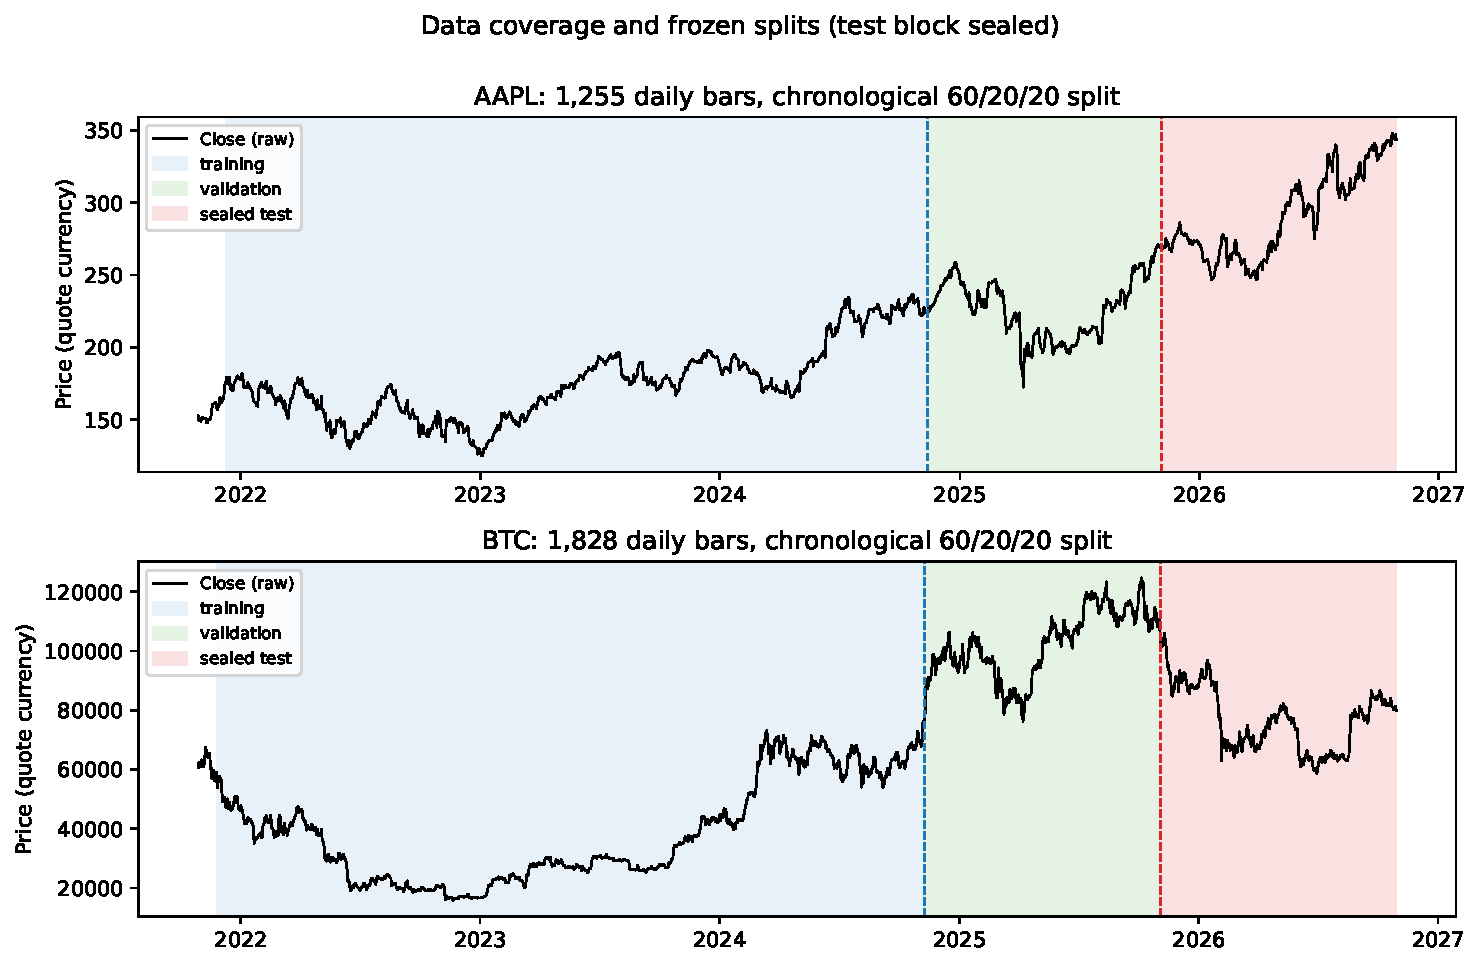
\includegraphics[width=0.9\linewidth]{figures/fig01_coverage_and_splits.pdf}
  \caption{Price history with the fixed 60/20/20 chronological split. Blue is
  training, green validation, red the \textbf{sealed test block}, which no run has
  read. The unshaded start is the feature warm-up.}
  \label{fig:coverage}
\end{figure}

\begin{figure}[t]
  \centering
  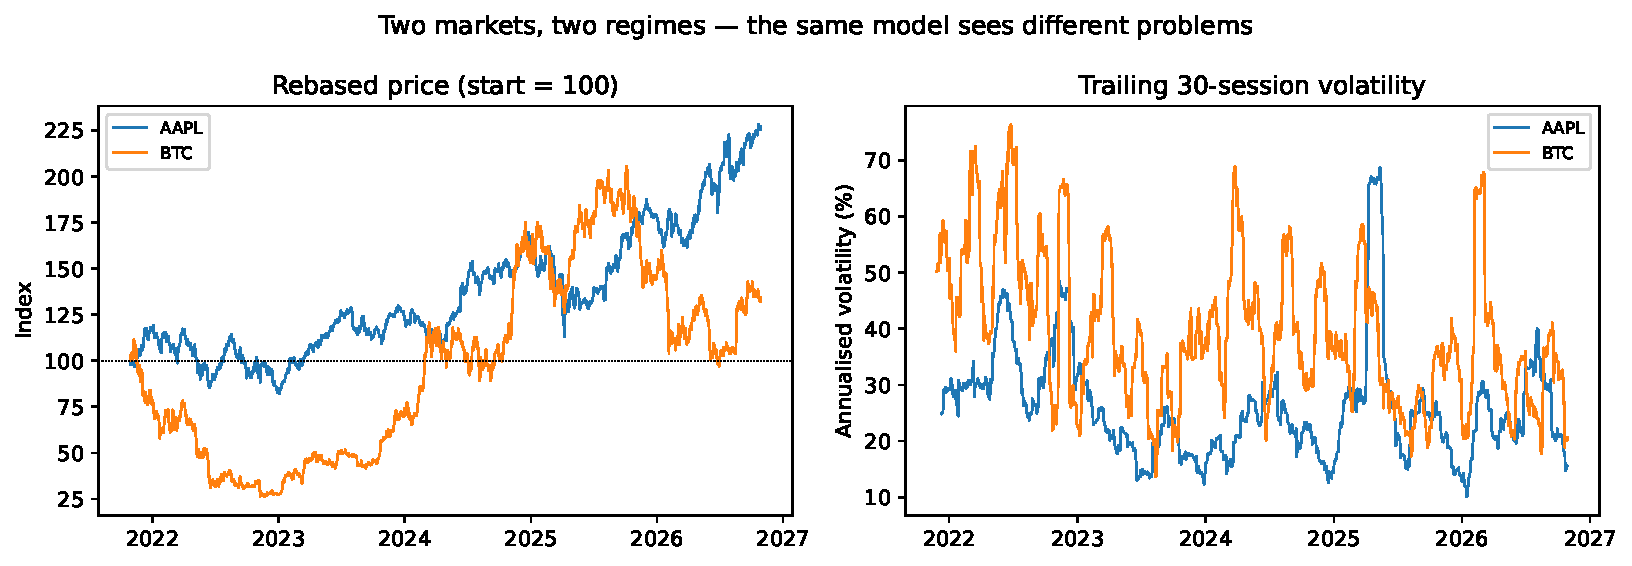
\includegraphics[width=0.9\linewidth]{figures/fig02_asset_characteristics.pdf}
  \caption{How the markets differ. Left: each series rebased to 100. Right:
  annualised 30-session volatility. BTC is usually more volatile.}
  \label{fig:assets}
\end{figure}

\section{Features and Leakage Control}
\label{sec:features}

The ten features are trailing ratios: returns over 1, 5 and 20 sessions; gaps to
5- and 20-session moving averages; realised volatility over 10 and 30 sessions;
intra-bar range; a volume anomaly; and day of week. Each uses bars up to and
including $t$, and rolling statistics require a full window.

Features are \emph{scale free} rather than price levels, which are non-stationary
and would let a model look accurate by copying today's price. The
reported quantity is error on the next close \emph{price}, while models are fitted
on the price \emph{change} and reconstructed as
$\hat{C}_{t+1} = C_t + \widehat{\Delta}_t$. The two are information-equivalent
because $C_t$ is known at decision time.

\paragraph{Boundary purge.}
With $y_t = C_{t+1}$, the last training label is a validation price and the last
validation label a sealed test price, so one row is dropped at each boundary. An
independent audit showed that, without it, perturbing one test price moved the
headline metric by 0.408 (Table~\ref{tab:splits}).

% GENERATED by scripts/build_latex_assets.py -- do not edit by hand.
\begin{table}[t]
\centering
\caption{Chronological split boundaries in the asset's own calendar. One row is purged at each boundary so that no label crosses a split: with $y_t = C_{t+1}$, the last training label would otherwise be a validation price and the last validation label a sealed test price. The test block remains unopened.}
\label{tab:splits}
\small
\setlength{\tabcolsep}{4pt}
\begin{tabular}{@{}l l l l r@{}}
\toprule
Asset & Training & Validation & Sealed test & Total \\
\midrule
AAPL & 2021-12-10..2024-11-08 & 2024-11-12..2025-11-03 & 2025-11-05..2026-10-27 & 1,224 \\
BTC & 2021-11-27..2024-11-07 & 2024-11-09..2025-11-01 & 2025-11-03..2026-10-28 & 1,797 \\
\bottomrule
\end{tabular}
\par\smallskip\footnotesize
Total is the number of usable feature rows after the trailing-window warm-up and the terminal unlabelled row are removed.
\end{table}


\paragraph{Enforcement.}
One test recomputes every feature from raw data with trailing formulas written
separately in the test, so a forward peek mismatches; another appends absurd future
prices and asserts earlier values are unchanged. Six canonical defects --- a
one-bar forward shift, an obfuscated equivalent, a centred window, a backward
fill, a whole-series statistic, and preprocessing fitted on train-plus-test ---
are then injected one at a time, and each must be detected.

\section{Experimental Methodology}
\label{sec:method}

Each asset is split chronologically into 60\% training, 20\% validation and 20\%
sealed test on its own session index, with a one-row purge at each boundary
(Table~\ref{tab:splits}); all models see identical boundaries and dates. Hyperparameters are chosen by random search inside an
expanding-window time-series cross-validation confined to the training block:
five folds, a one-fold gap, minimum initial training fraction 0.30. Because
tuning never sees validation, validation remains a selection holdout rather than
a second tuning set. Every family gets the same budget, \TrialsUsed{} trials and at most \SecondsUsed{}~s
per cell (the protocol caps \TrialsMax{} and \SecondsMax{}~s), and every attempted
configuration is logged.

\begin{figure}[t]
  \centering
  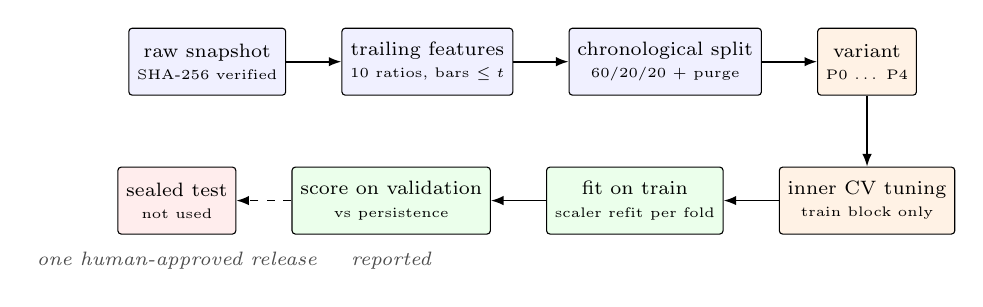
\begin{tikzpicture}[
      node distance=5mm and 7mm,
      box/.style={draw, rounded corners=1.2pt, align=center, font=\scriptsize,
                  inner sep=3pt, minimum height=8.5mm},
      arr/.style={-{Latex[length=1.6mm]}, semithick},
      lbl/.style={font=\scriptsize\itshape, text=black!70}]
    \node[box, fill=blue!6] (raw) {raw snapshot\\{\tiny SHA-256 verified}};
    \node[box, fill=blue!6, right=of raw] (feat) {trailing features\\{\tiny 10 ratios, bars $\le t$}};
    \node[box, fill=blue!6, right=of feat] (split) {chronological split\\{\tiny 60/20/20 + purge}};
    \node[box, fill=orange!10, right=of split] (pre) {variant\\{\tiny P0 \dots\ P4}};
    \node[box, fill=orange!10, below=9mm of pre] (tune) {inner CV tuning\\{\tiny train block only}};
    \node[box, fill=green!8, left=of tune] (fit) {fit on train\\{\tiny scaler refit per fold}};
    \node[box, fill=green!8, left=of fit] (eval) {score on validation\\{\tiny vs persistence}};
    \node[box, fill=red!7, left=of eval] (test) {sealed test\\{\tiny not used}};

    \draw[arr] (raw) -- (feat);
    \draw[arr] (feat) -- (split);
    \draw[arr] (split) -- (pre);
    \draw[arr] (pre) -- (tune);
    \draw[arr] (tune) -- (fit);
    \draw[arr] (fit) -- (eval);
    \draw[arr, dashed] (eval) -- (test);
    \node[lbl, below=1mm of eval] {reported};
    \node[lbl, below=1mm of test] {one human-approved release};
  \end{tikzpicture}
  \caption{The experiment pipeline, drawn to match the implementation. The scaler
  is fitted \emph{inside} the model pipeline, so it is refitted per fold and
  cannot see validation rows. Dashed arrow: the test block is not evaluated by
  any run in this report.}
  \label{fig:pipeline}
\end{figure}

We report MAE, RMSE and $R^2$, plus \emph{skill} relative to persistence on
identical forecast dates:
\begin{equation*}
  \text{skill}_{\text{MAE}} \;=\; 1 - \frac{\text{MAE}_{\text{model}}}{\text{MAE}_{\text{naive}}}.
\end{equation*}
Skill is primary because it has a meaningful zero. $R^2$ is inflated on a trending level: our naive forecast itself attains $R^2 \approx 0.96$, so a high $R^2$
here indicates a trending series, not a good model. Absolute errors are never
compared across assets. Uncertainty uses a moving-block bootstrap over consecutive dates; overlapping blocks retain dependence, so we treat it as indicative only.

\section{Model Selection and Baselines}
\label{sec:models}

The five families differ in mechanism rather than to reach a count: a
near-unregularised linear model as a learned floor, Ridge as a regularised linear
reference, RBF support vector regression as a kernel method, a random forest as a
bagged ensemble, and histogram gradient boosting as a boosted ensemble. A shallow neural network was considered and left gated: the written handout
discourages deep learning, and the instructor's reported oral guidance is recorded
as reported guidance, not as a changed rule, so that lane does not appear here.

The mandatory baseline is naive persistence, $\hat{C}_{t+1} = C_t$. It is not a straw man: for a near-random-walk series it is strong, free, and
defines the zero of the skill scale \citep{makridakis2018m4,hyndman2021fpp3}. Forecasting competitions reach the same conclusion
about simple benchmarks \citep{makridakis2018m4,hyndman2021fpp3}.

Every family is built through one shared code path, so each receives identical
feature columns in identical order and any scaler sits inside its pipeline where
it is refitted per fold. Tests assert that column identity and that a fixed seed
is deterministic.

\section{Preprocessing Ablation}
\label{sec:ablation}

RQ3 asks how much preprocessing matters. We vary one factor at a time, holding
model, features, split and tuning budget fixed; the contrast is scaling, with P0
unscaled and P2 standardised on training rows only.

% GENERATED by scripts/build_latex_assets.py -- do not edit by hand.
\begin{table}[t]
\centering
\caption{Controlled preprocessing ablation: validation MAE without standardisation (P0) and with it (P2), holding model, features, split and tuning budget fixed. A change of exactly $0.000\%$ means the model is invariant to monotone per-feature rescaling, which is the theoretical prediction for tree ensembles and serves as a negative control.}
\label{tab:ablation}
\small
\setlength{\tabcolsep}{4pt}
\begin{tabular}{@{}l r r r r r@{}}
\toprule
 & \multicolumn{3}{c}{AAPL} & \multicolumn{2}{c}{BTC} \\
\cmidrule(lr){2-4}\cmidrule(l){5-6}
Model & P0 MAE & P2 MAE & $\Delta$ & P0 MAE & $\Delta$ \\
\midrule
Linear baseline & 2.899 & 2.920 & +0.745 & 1600.205 & +0.211 \\
Ridge & 2.898 & 2.897 & -0.041 & 1601.874 & +0.032 \\
SVR (RBF) & 2.891 & 2.890 & -0.010 & 1604.186 & -0.066 \\
Random forest & 2.928 & 2.928 & \textbf{0.000} & 1603.373 & \textbf{0.000} \\
Hist.\ gradient boosting & 2.898 & 2.898 & \textbf{0.000} & 1605.016 & \textbf{0.000} \\
\bottomrule
\end{tabular}
\par\smallskip\footnotesize
$\Delta$ is the percentage change in validation MAE from P0 to P2. Bold $0.000$ denotes bit-identical predictions.
\end{table}


The measured pattern matches Section~\ref{sec:background}, exactly rather than
approximately: for both tree ensembles the change in validation MAE is
\emph{bit-identical} --- $0.000\%$ to printed precision --- on both assets. That is a strong internal control: had scaling moved the forests, the correct
inference would be a bug, not a discovery.

Scaling-sensitive families move slightly and not uniformly helpfully:
standardisation barely changes AAPL Ridge, worsens the AAPL linear baseline
(Table~\ref{tab:ablation}) and rescues nothing --- every value stays within about
one percentage point of the baseline. An ablation ending in no
substantial effect is a legitimate finding, and a useful teaching one: it
separates \emph{this transform changes the model} from \emph{this transform
improves the forecast}.

One variant is reported as not run: with no missing values in either snapshot an
imputation variant would duplicate the baseline cell, and we did not inject
synthetic gaps to manufacture a contrast.

\begin{figure}[t]
  \centering
  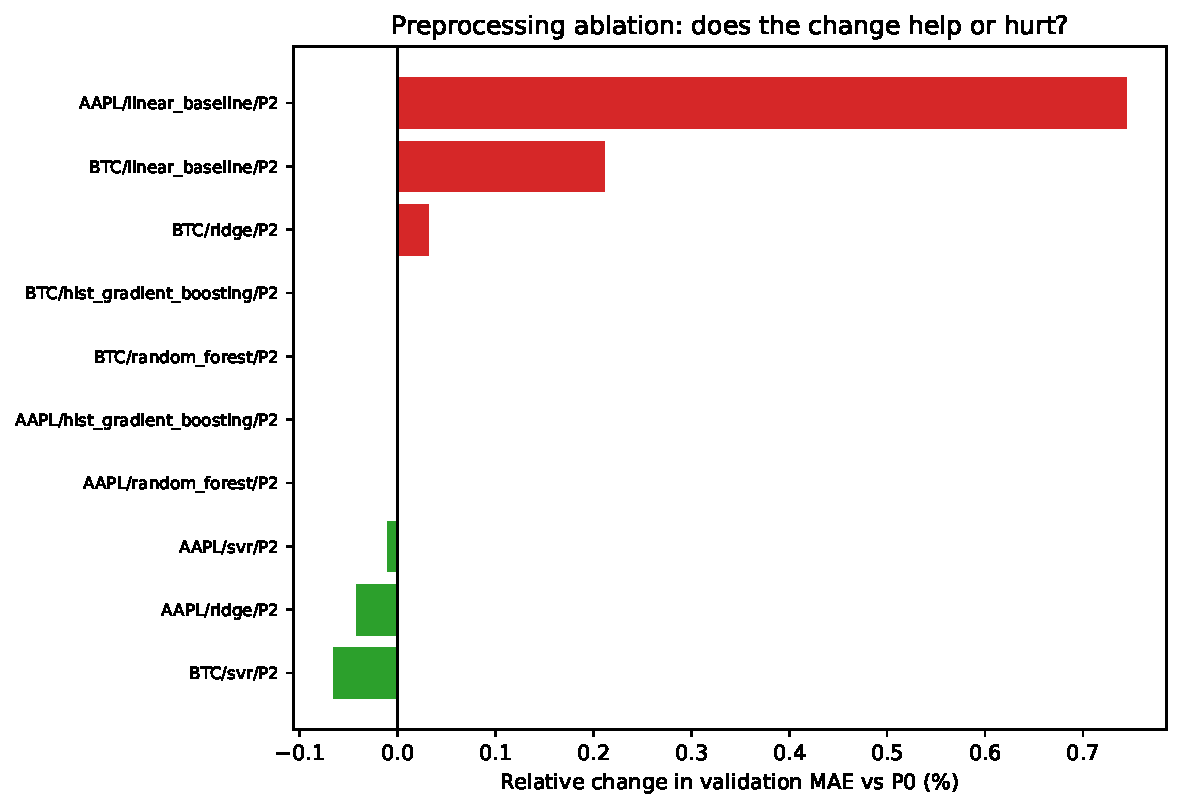
\includegraphics[width=\linewidth]{figures/fig06_ablation_delta.pdf}
  \caption{Relative change in validation MAE between unscaled (P0) and
  standardised (P2) variants, holding model and asset fixed. Bars at exactly zero
  are the tree ensembles, whose predictions are bit-identical under monotone
  rescaling. Only matched cells are plotted.}
  \label{fig:ablation}
\end{figure}

\section{Evaluation and Results}
\label{sec:results}

Table~\ref{tab:results} reports validation performance; all \NRunTotal{} runs
completed successfully and none read the test block.

% GENERATED by scripts/build_latex_assets.py -- do not edit by hand.
% Source: experiments/models/*/*/metrics.json (validation split only).
\begin{table}[t]
\centering
\caption{Validation performance for each model family under the shared protocol (variant P2, standardised inputs, seed 42). Skill is measured against naive persistence on identical forecast dates. Absolute errors are in quote currency and are \emph{not} comparable between AAPL and BTC; only the unitless skill column is. The test block was not used.}
\label{tab:results}
\small
\setlength{\tabcolsep}{4pt}
\begin{tabular}{@{}l r r r r r r@{}}
\toprule
 & \multicolumn{3}{c}{AAPL} & \multicolumn{3}{c}{BTC} \\
\cmidrule(lr){2-4}\cmidrule(l){5-7}
Model & MAE & RMSE & Skill & MAE & RMSE & Skill \\
\midrule
Linear baseline & 2.92 & 4.37 & \textbf{-0.50} & 1603.59 & 2211.24 & +0.05 \\
Ridge & 2.90 & 4.36 & +0.29 & 1602.39 & 2205.96 & +0.12 \\
SVR (RBF) & 2.89 & 4.36 & +0.52 & 1603.13 & 2203.85 & +0.08 \\
Random forest & 2.93 & 4.37 & \textbf{-0.78} & 1603.37 & 2208.04 & +0.06 \\
Hist.\ gradient boosting & 2.90 & 4.36 & +0.25 & 1605.02 & 2204.91 & \textbf{-0.04} \\
\midrule
Naive persistence & 2.91 & 4.36 & 0.00 & 1604.35 & 2205.67 & 0.00 \\
\bottomrule
\end{tabular}
\par\smallskip\footnotesize
Skill is $1 - \mathrm{MAE}_{\mathrm{model}}/\mathrm{MAE}_{\mathrm{naive}}$ in percent; negative values (bold) are worse than the baseline. $n=244$ (AAPL) and $358$ (BTC) validation sessions.
\end{table}


\paragraph{RQ1: nothing meaningfully beats persistence.}
The best result is \BestAAPLModel{} on AAPL at \BestAAPLSkill\% skill and
\BestBTCModel{} on BTC at \BestBTCSkill\% --- a fraction of a percentage point
above doing nothing. Two models are worse: the random forest on AAPL
(\SkillAAPLRandomForest\%) and the boosted ensemble on BTC
(\SkillBTCHistGradientBoosting\%).
\begin{figure}[t]
  \centering
  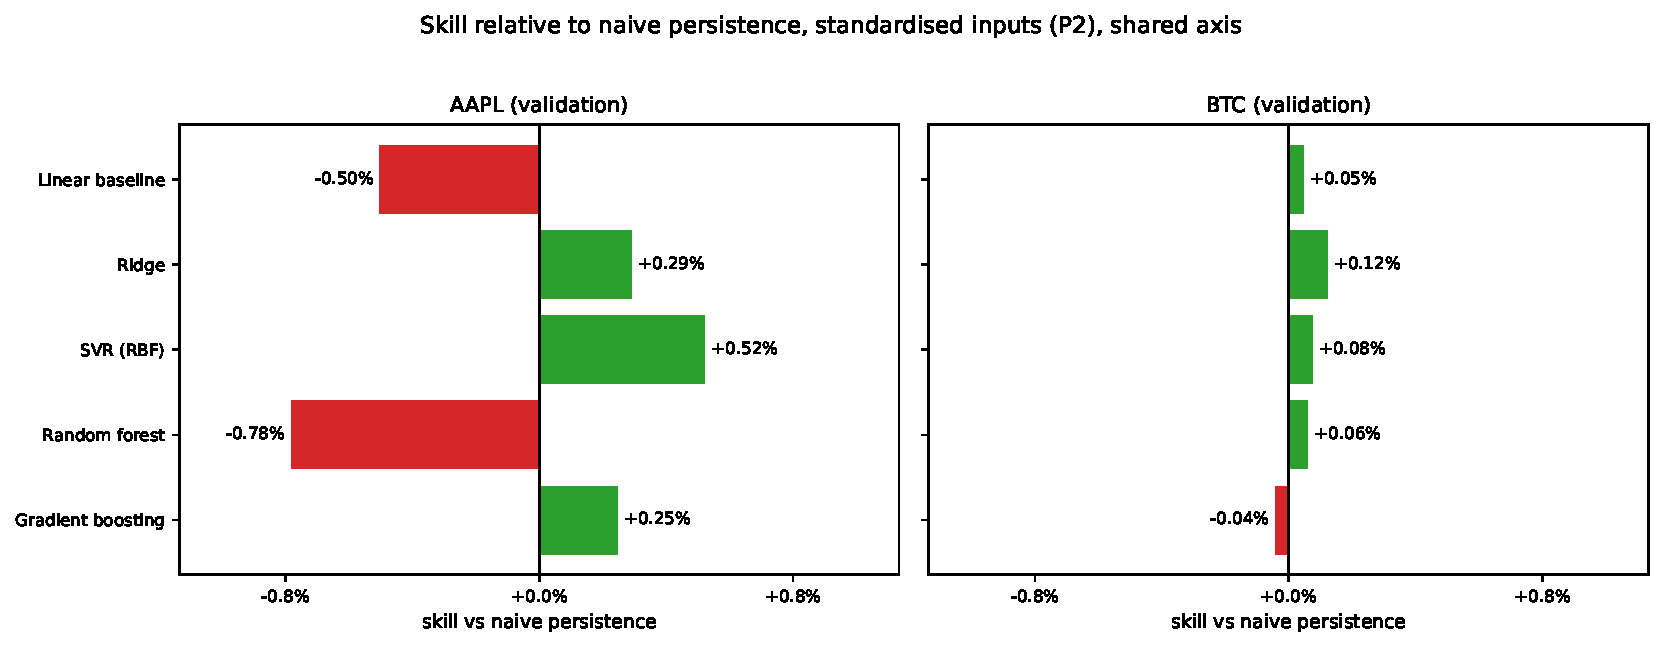
\includegraphics[width=\linewidth]{figures/fig04_model_vs_naive.pdf}
  \caption{Skill relative to naive persistence, per asset, on a \emph{shared}
  horizontal axis. Sharing matters: per-panel autoscaling would make BTC's
  fraction of a percent look as large as AAPL's. Bars left of zero are worse than
  repeating the current price.}
  \label{fig:skill}
\end{figure}

\paragraph{RQ2: capacity and regimes.}
Figure~\ref{fig:assets} gives the mechanical explanation: BTC's volatility is
higher and more variable, so a model with capacity fixed by an identical budget
faces a harder target, and every BTC skill value is closer to zero. On AAPL, where
capacity has more room to matter, the most flexible ensemble does worst --- the
signature of fitting noise.

\begin{figure}[t]
  \centering
  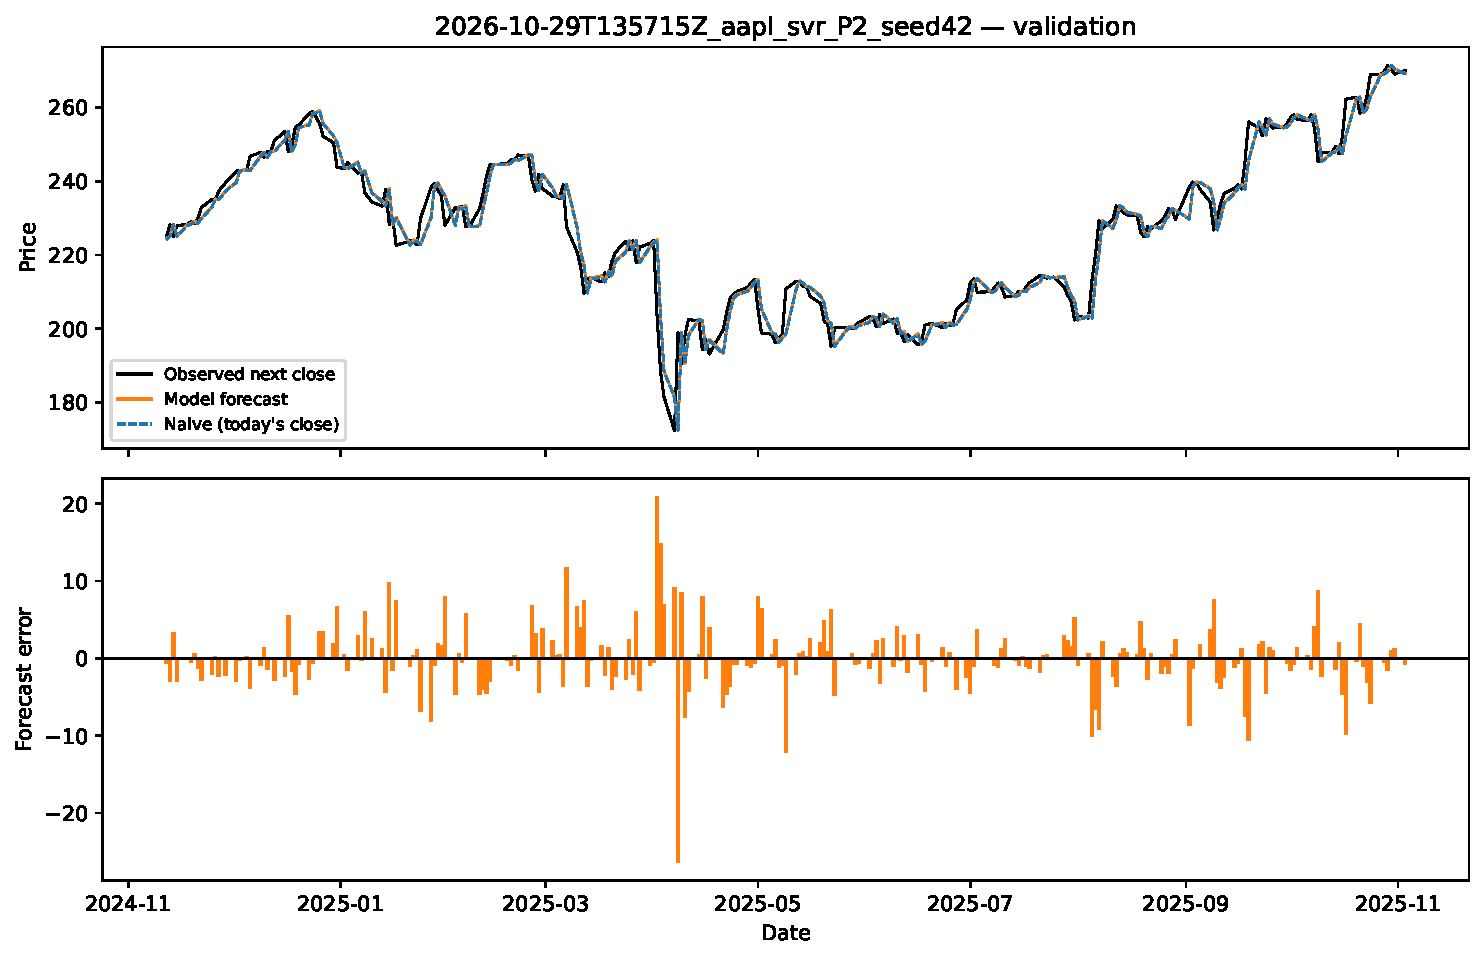
\includegraphics[width=0.78\linewidth]{figures/fig03_observed_vs_predicted_2026-10-29T135715Z_aapl_svr_P2_seed42_validation.pdf}
  \caption{Observed next close against the fitted SVR and naive forecasts on the
  AAPL validation block, with signed error below. The naive line tracks the
  observed series closely, which is why absolute error is a poor way to judge a
  model and skill is used instead.}
  \label{fig:forecast}
\end{figure}

\paragraph{Why they fail.}
The explanation is statistical, not architectural: daily return autocorrelation is
close to zero, so the features carry little information about the next session's
direction and extra parameters fit noise. The forest adds a structural limit ---
its predictions average leaf values, so it cannot extrapolate. Since all skill values lie within about one percentage point and the middle
ranking changes between assets, we claim no family is superior: the conclusion is
a tie against the baseline.

\begin{figure}[t]
  \centering
  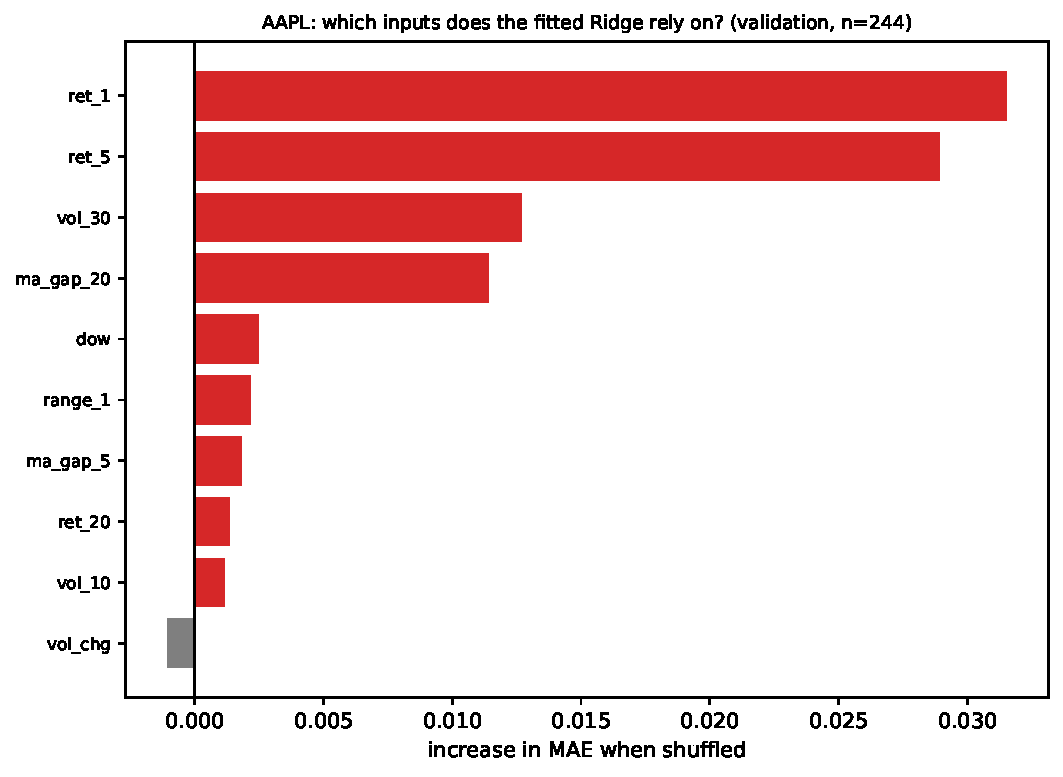
\includegraphics[width=0.76\linewidth]{figures/fig07_feature_importance_aapl.pdf}
  \caption{Learner-facing interpretability: permutation importance for the fitted
  Ridge model on the AAPL validation block, measured as the increase in MAE when
  one feature is shuffled \citep{fisher2019allmodels}. The model relies most on short-horizon returns and
  trailing volatility, and the magnitudes are tiny --- consistent with the skill
  table. This describes the fitted model, not a causal claim about markets.}
  \label{fig:importance}
\end{figure}

\section{Neural Networks (Experimental)}
\label{sec:dl}

Outside the main protocol, an MLP on the ten features and an LSTM on their last 20
days \repofile{scripts/supplementary_direction_test.py}{predicted next-day
direction}. We tuned them on the end of the training block and averaged over
\SupSeeds{} seeds (Table~\ref{tab:dl}). Training used Adam, batch size 64 and at
most \SupMaxEpochs{} epochs, with patience \SupPatience.

\begin{itemize}
  \item \textbf{AAPL:} both scored below ``always up''.
  \item \textbf{BTC:} both scored above ``always down'', but \textbf{all \SupNCi{}
  intervals include zero}.
  \item Hold-out log-loss (\SupLossLo--\SupLossHi) is close to the coin-flip value
  $\ln 2 \approx 0.693$.
\end{itemize}

\textbf{No clear evidence that these networks add predictive signal.}

% GENERATED by scripts/build_latex_assets.py -- do not edit by hand.
% Source: experiments/supplementary/direction_test/*/results.json (decision D14).
\begin{table}[t]
\centering
\caption{Experimental neural-network test: share of validation sessions whose next-day direction (up or not up) was called correctly. Seed range in brackets; interval = 95\% moving-block bootstrap of the difference from the majority rule, in percentage points. The LSTM reads a sequence, so its inputs differ from the main study.}
\label{tab:dl}
\small
\setlength{\tabcolsep}{4pt}
\begin{tabular}{@{}p{0.27\linewidth} p{0.33\linewidth} p{0.33\linewidth}@{}}
\toprule
 & AAPL & BTC \\
\midrule
Majority rule (from training) & always up: 55.7\% & always down: 48.0\% \\
MLP, today's 10 features & 54.1\% [48.4--57.8]; $-1.6$ ($-10.7$, $+7.0$) & 50.0\% [48.9--50.0]; $+2.0$ ($-4.8$, $+7.3$) \\
LSTM, last 20 days of features & 52.0\% [45.5--55.7]; $-3.7$ ($-11.9$, $+5.3$) & 53.3\% [49.2--52.0]; $+5.3$ ($-0.3$, $+10.1$) \\
Five classical models (range) & 50.4--58.6\% & 48.9--53.1\% \\
\bottomrule
\end{tabular}
\end{table}


\section{Educational Implications}
\label{sec:education}

RQ4 asks what these results can teach; the answer is a designed resource, not a
measured outcome. No learners were observed or surveyed, so these statements describe what a lesson
makes visible, not what anyone learned.

The lesson has five observable objectives: explain why a model that scores well
historically may fail tomorrow; identify leakage in a code fragment; interpret a
skill score including a negative one; predict which families are scale-sensitive
and justify it mechanistically; and distinguish forecast error from profitability.
Each is anchored to a real artefact: the negative random-forest entry in
Table~\ref{tab:results} is the teaching moment for the third, and
Figure~\ref{fig:ablation} asks why the tree bars are exactly zero.

Its most valuable property is that the headline result is negative. A demonstration
where the sophisticated model wins teaches that complexity is good; this one
teaches the transferable question \emph{what is the baseline, and did we beat it?}
Five formative tasks with worked answers accompany it, and the notebook lets a
non-specialist re-run the comparison.

\section{Limitations and Threats to Validity}
\label{sec:limitations}

\paragraph{Scope and target.}
Two assets, one window, one horizon, one convention. BTC is a single venue's USDT
price, not a global index. The label is the raw close one session ahead, so
dividends are ignored, and a one-session horizon is where persistence is
strongest --- a bias against trained models that follows from the question we
chose, and the reason H1 was pre-registered rather than discovered.

\paragraph{Statistics and evaluation integrity.}
Skill differences are within about one percentage point and intervals overlap, so
we report a tie; because errors are serially dependent, even block resampling
understates uncertainty. Every number here is a validation number, and validation
influenced model selection, so it is not a clean holdout; the sealed block exists
to give one unbiased estimate once the analysis is frozen.

\paragraph{Measurement integrity.}
Two leakage defects were found by independent audit and fixed. Both would have inflated results, and both were invisible to the authors of the
code: the audit mechanism, not the initial implementation, is what makes these
numbers trustworthy.

\paragraph{Education.}
No learner study was run, so claims about the lesson are design claims.

\section{Challenges and Team Learnings}
\label{sec:learnings}

The first challenge was target representation. Initial runs reported skill near
$-1800\%$. The features contained no price level, so the models could not recover
it and collapsed towards the training mean. After seeing this, we changed the
training target to the price change and recorded the decision.

The second was the boundary purge, found when an auditor traced a label to a test
price. Our first leakage tests had also passed with a one-bar forward shift
present. A passing test suite means more once it has been shown able to fail.

The third was fairness. Sharing one construction path, tuning budget and feature
set took more effort than fitting the models, but it made the comparison
meaningful.

\section{Conclusion}
\label{sec:conclusion}

Under a documented, leakage-audited protocol, none of five models meaningfully or
consistently outperformed a one-line persistence rule at predicting the next close
of Apple and Bitcoin. The best skill was \BestAAPLSkill\%, \NBelowAll{} of
\NRunTotal{} runs were worse than the rule, and the experimental networks showed no
clear advantage on direction.

For this course, the negative result supports the main lesson: ask of any model
what it beat, and how you know. The repository lets readers check the claim.
Nothing here is investment advice, and we have not measured learning gains.




\section*{Acknowledgements}
\addcontentsline{toc}{section}{Acknowledgements}
\noindent The repository holds hashed data snapshots, the protocol, run manifests,
tests and the notebook. AI coding assistants (Pi with
\texttt{pi-subagents}, and Claude Code) drafted code, tests and text under a
documented protocol. Zhang Yancheng directed that work: he
set the research direction, made the final decisions, and reviewed and verified
every AI-assisted change. This work is
educational, not investment advice.

\bibliographystyle{plainnat}
\bibliography{references}

\end{document}
